\documentclass[a4paper,twoside,notitlepage,11pt]{article}
\usepackage{graphicx}
\usepackage{hyperref}
\usepackage{fancyeq}
\usepackage{amstext}
\usepackage{tabularx}
\usepackage{amssymb}
\usepackage{longtable}
\usepackage{fancyhdr}
\usepackage{multirow}
\usepackage{tocloft}
\usepackage{lscape}
\usepackage{transparent}
\usepackage{subcaption}
\usepackage{rotating}
\usepackage{titletoc}
\usepackage{setspace}
\usepackage[all]{xy}
\usepackage{nccmath}
\usepackage[a4paper,hmargin=2.5cm,vmargin=2.5cm]{geometry}
\usepackage[hypcap]{caption}
\usepackage{qtree}
\usepackage{cleveref}
\usepackage{mathpartir}
\usepackage{listings}
\usepackage{multirow}
\usepackage{enumitem}
\usepackage{float}
\usepackage[compact]{titlesec}
\usepackage{layouts}
\usepackage{wrapfig}
\usepackage{listings}
\usepackage{color}
\usepackage{xcolor}

\hypersetup{
    unicode=false,
    pdftoolbar=true,  
    pdfmenubar=true,     
    pdffitwindow=false,    
    pdfstartview={FitH},  
    pdftitle={Title},  
    pdfauthor={Craig Knott},
    pdfsubject={CS},
    pdfnewwindow=true,  
    colorlinks=true,  
    linkcolor=black,  
    citecolor=black, a
    filecolor=black,  
    urlcolor=black  
}

\newcommand{\paperTitleShort}{Niceway.to: Scenic Route Mapping}
\newcommand{\paperTitle}{Niceway.to: Scenic Route Mapping}

\newcommand{\nocontentsline}[3]{}
\newcommand{\tocless}[2]{\bgroup\let\addcontentsline=\nocontentsline#1{#2}\egroup}

\newenvironment{changemargin}[2]{%
\begin{list}{}{%
\setlength{\topsep}{0pt}%
\setlength{\leftmargin}{#1}%
\setlength{\rightmargin}{#2}%
\setlength{\listparindent}{\parindent}%
\setlength{\itemindent}{\parindent}%
\setlength{\parsep}{\parskip}%
}%
\item[]}{\end{list}}

\setlength{\parskip}{0.25em}

\renewcommand{\headrulewidth}{0.0pt}

\fancypagestyle{plain}{
	\fancyhf{}
	\fancyhead[LO]{Craig Knott}
	\fancyhead[CO]{\textit{\paperTitleShort}}
	\fancyhead[RO]{\thepage}
	\fancyhead[LE]{\thepage}
	\fancyhead[CE]{\textit{\paperTitleShort}}
	\fancyhead[RE]{Craig Knott}
}

\fancypagestyle{appendix}{
	\fancyhf{}
	\fancyhead[LO]{Craig Knott}
	\fancyhead[CO]{\textit{\paperTitleShort}}
	\fancyhead[RO]{\thepage}
	\fancyhead[LE]{\thepage}
	\fancyhead[CE]{\textit{\paperTitleShort}}
	\fancyhead[RE]{Craig Knott}
}

\fancypagestyle{biblio}{
	\fancyhf{}
	\fancyhead[LO]{cxk01u}
	\fancyhead[CO]{\textit{\paperTitleShort}}
	\fancyhead[RO]{\thepage}
	\fancyhead[LE]{\thepage}
	\fancyhead[CE]{\textit{\paperTitleShort}}
	\fancyhead[RE]{Craig Knott}
}

\begin{document}

%
%
% Title Page
%
%

\pagestyle{empty}
\newgeometry{left=99pt, right=99pt, top = 75pt, bottom=75pt}
\begin{center}
\ \\[1cm]
\LARGE{\textbf{\paperTitleStart}}\ \\[0.5cm]
\large{Submitted March 2016 in partial fulfilment of the conditions of the award of the degree MSci (Hons) Computer Science}
\ \\[1cm]
\large{\textbf{Craig Knott}} \ \\
\large{cxk01u}\ \\[0.3cm]

With Supervision from Max L. Wilson\\[0.3cm]

School of Computer Science and Information Technology \ \\
University of Nottingham \ \\
 \ \\[0.5cm]
I hereby declare that this dissertation is all my own work, except as indicated in the text: \ \\[1cm]
\end{center}

\begin{Large}
\begin{center}
\begin{tabular}{l}
Signature \rule{5cm}{1pt} \ \\[0.2cm]
\end{tabular}
\end{center}

\begin{center}
\begin{tabular}{l}
Date \rule{1.5cm}{1pt}/\rule{1.5cm}{1pt}/\rule{1.5cm}{1pt}\ \\
\end{tabular}
\end{center}
\end{Large}

\ \\[0.6cm]
\begin{center}
\includegraphics[scale=0.55]{images/UoN_Arms}
\end{center}
\cleardoublepage

%
%
% Abstract
%
%

\begin{abstract}
{\color{red} Project abstract}
\end{abstract}

\null
\vfill
\begin{flushright}
	\begin{tabular}{r|l}
		Words in text	& 19,552 \\
	\end{tabular}
	\ \\
	\ \\
	\begin{tabular}{cc}
		\multicolumn{2}{r}{Calculated with the TeXCount web service}\\
		\multicolumn{2}{r}{\url{http://app.uio.no/ifi/texcount/online.php}}
	\end{tabular}
\end{flushright}

\cleardoublepage

%
%
% Table of Contents
%
%


\newgeometry{left=3cm, right=3cm, top = 75pt, bottom=75pt}
\setlength{\cftbeforesecskip}{0.6ex}
\addtocontents{toc}{\protect\thispagestyle{empty}}
\tableofcontents
\cleardoublepage

%
%
% Sections 
%
%

\newpage
\pagestyle{plain}
\setcounter{page}{1}

\section{Introduction}
In recent years, the technologies behind satellite navigation and routing services have greatly advanced, allowing them to produce the quickest route between two points without spending more than a few seconds calculating it, even with technological limits \cite{lou2009map}. As a result, travelling via car is quicker and easier than ever before, and many drivers have now become focussed simply on reaching their destination as quickly as possible. This has resulted in a shift in the mindset of society where the scenery that we pass on the roads is simply a buffer between segments of our day, and it's beauty is left unappreciated. This mentality promotes a  culture of instant gratification, impatience, and self-involvement among the driving community, which has a huge detrimental affect on drivers, where any interruptions on their journey are cause for anger. In fact, it has been shown that since 1990 incidents of aggression during driving has risen 51\% \cite{vest1997road}. \ \\
\ \\
Some research has already been completed in an attempt to shift the focus of driving from simply travel, to also being an enjoyable recreational activity. This includes work such as automatically determining how ``nice'' a route is, using social network data \cite{peregrino2012mapping}\cite{van2011time} and how to personalise routes that have been deemed ``efficient'' \cite{chen2011discovering}. Outside of the world of research, many services already exist that provide users with a collection of scenic routes between two locations. The purpose of these services is to encourage drivers to enjoy driving more, and experience more of their surroundings. Examples of these include Google's ``My Maps''\cite{url2015gmaps}, MADMAPS\cite{url2015madmaps}, and MyScenicDrives\cite{url2015myscenicdrives}, which are discussed in further detail in section \ref{sec:existing-systems}.\ \\
\ \\
Unfortunately, these systems have some flaws that mean they do not wholly solve this problem, and therefore have not made a huge impact. The largest two being the method of delivery, and lack of user contribution (for MADMAPs and MyScenicDrives). These services are optimised for desktop browsing, and do not function well on mobile devices which, considering that in the UK 33\% of Internet users believe their smartphones to be the most important device for going online\cite{ofcom2015comms}, is a large portion of users lost. Alongside these major flaws, some other minor flaws are also present, including primitive search functionality, a small user base, slow and unresponsive webpages, and some services costing money.\ \\
\ \\
Niceway.to is a service with three main aims: to build a community of travel enthusiasts, improve the travelling experience of those that use it, and allow for users of all skill groups to access it. It provides a way for users to discover scenic and visually interesting routes between two locations, all of which have been provided by other members of the community. These routes will each contain a social commentary, with users being able to rate, comment on, and share (this will  be an incentive for users to provide quality content, and to remain loyal to the site). To address the problem of previous software systems, mainly the method of delivery, it is built as a fully-responsive web-application that functions equally well on desktop and mobile devices. \ \\
\ \\
As a final note, it is worth mentioning that this project will not focus on the classification of whether or not routes are ``nice'' or ``scenic''. Instead, the content will be entirely user driven, with the assumption that they would only contribute routes that are interesting and visually appealing. To further encourage this, a rating system for routes will be implement, so that ``better'' routes are more visible than those deemed less so.

\newpage 
\section{Motivation}
Niceway.to is an application envisioned by my client, Matthew Pike, who works for a small start-up in China. The project has already been worked on once before, but the end result was not to a standard that my client was content with. As a result of this, he would like for the project to be redesigned and recreated from scratch, as little of the original software is reusable.\ \\
\ \\
The main motivation of this project is to change how we think about driving: from simply a tool for travel, to an enjoyable recreational activity, where, instead of being focused solely on reaching our destination, we can take time to appreciate the beauty in the world around us. In a 1995 study, almost 90\% of motorists had experienced some form of road rage within the preceding 12 months, and 60\% admitted to losing their temper whilst behind the wheel\cite{joint1995road}. To facilitate this proposed shift in mentality, this project will be a tool that offers a collection of user submitted scenic driving routes, with a heavy focus on utilising the social characteristics of the Internet. The idea being that when a user wishes to travel somewhere, they could do so by travelling a route lesser known to them. This route may be slower, but would make up for the time lost, by providing a visually enriching experience that the driver would have otherwise been deprived of, and to help avoid common annoyances on the road. This would also help to relieve the monotony of driving the same, mundane, routes repeatedly - which has been shown to have serious implications in terms of accident causation\cite{thiffault2003monotony}. \ \\
\ \\
A big part of this project, which my client has stressed, is to foster a community of travel enthusiasts. Specifically the ability to have a social commentary surrounding each route, where registered users of the application are able to express their opinions on the content, give a numeric rating for the content, as well as share the content (both internally and externally). The reason for this is because a user is far more likely to return to, and remain engaged with, a website if there are other users doing the same, especially if they are directly communicating with those other users\cite{ling2005using}. Allowing users to submit their own content coaxes them into feeling more of a connection to the site, and will increase their chance of returning (so that they can check how well received their content is). It has been shown that feedback is a useful tool to boost engagement\cite{o2008user} and hopefully this will encourage users to associate the site with positive experiences, and inspire them to produce quality content (in order to receive more of this feedback).\ \\
\ \\
In order for this community to thrive, it is vital that the system is simple to use, open to users of all skill groups, and easy to access. Therefore, it is important that HCI principles are kept in mind throughout every step of the design and implementation processes. Key to a good design, is simplicity. This is because complex user interfaces frustrate users, and can deter them from returning. Studies have shown that users lose more than 40\% of their time to frustration, and in most cases the user ends up angry at themselves, angry at the computer, or left with a feeling of helplessness\cite{lazar2006workplace}.\ \\
\ \\
In addition to all of these reasons, I feel personally motivated to ensure that this project succeeds. As someone who does not currently drive, I find myself in need of others to drive me when public transport proves inadequate. As a passenger, I will often observe the driver becoming evermore agitated with other drivers on the road, and seeing this problem first hand helps enforce my feelings of the importance of solving it. Driving is a freedom, but one that is being squandered and perceived more as a chore than an enjoyable activity.
\newpage 
\section{Background Information \& Research}
This sections look at some software systems that are already attempting to solve the problem identified in this dissertation, as well as discussing some of the different technologies considered for the implementation of this project.

\subsection{Existing Systems}
\label{sec:existing-systems}
As mentioned in section \ref{sec:intro}, software systems for the distribution and sharing of scenic routes already exist. Each of these systems approaches the problem in a different way, and thus all have their own advantages and disadvantages, which will be discussed here. The aim of this is to determine the best features and the worst features, so they can be incorporate or avoided.

\paragraph{Google's ``My Maps'', \url{https://www.google.com/maps/d}}\ \\
Google's ``My Maps'' service (distinct from ``Google Maps'') is a tool that offers users the ability to plot maps between locations, and save them to their Google accounts. This allows users to quickly access routes they travel frequently, as well share those routes with others (over various social media platforms). The main advantages of this service are that it provides a graphical tool for visualising routes, the ability to add photos and videos to specific waypoints, and, as mentioned above, the ability to share routes via social media. Another interesting feature that is provided is the ability to plot all the point, and generate the route afterwards, rather than generating the route after each point is placed. This is an interesting consideration for a mobile application, because users may wish to save on data (although if users are unaware of this being the reason, it just makes the tool look less responsive).\ \\
\ \\
The key disadvantage of Google's ``My Maps'' is that it is very slow, and there are long periods of loading in-between successive actions. Responsiveness on websites is key, otherwise users are unaware if their actions are having an impact or not. There are also other disadvantages, including the unintuitive and cluttered user interface, the small user base (being a relatively unknown piece of software, dwarfed by the Google Maps service), and that the only way of sharing your routes is to other social media platforms. This last point is particularly important to address for Niceway.to, because it aims is to build a community of users. If they can only share their routes to \textit{other} platforms, the community will have a much smaller chance of thriving. This is why all routes on Niceway.to will be accessible and searchable from within the system itself, and the sharing of routes will simply be a tool to draw more people to the site.

\begin{figure}[!ht]
	\begin{center}
		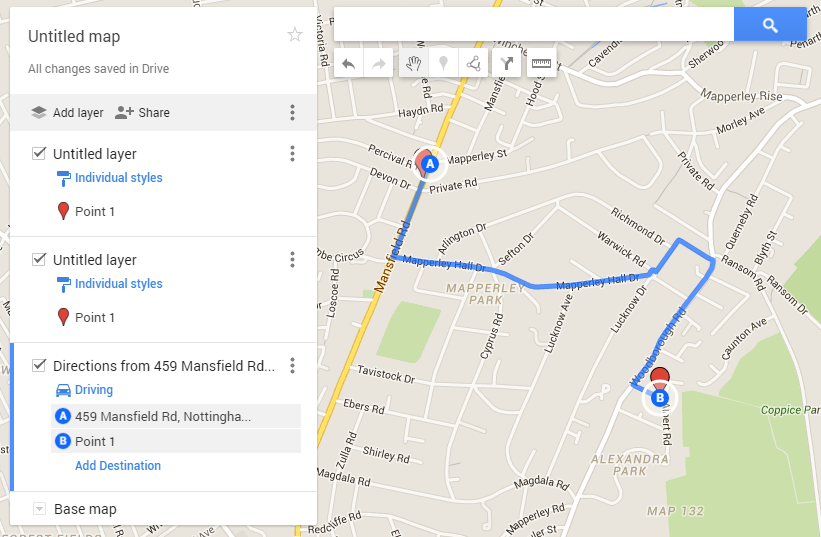
\includegraphics[width=0.66\textwidth]{images/background/gm_rcp.png}
	\end{center}
	\vspace{-6mm}
	\caption{Google's ``My Maps'' route creation/editing feature}
	\vspace{-6mm}
\end{figure}

\newpage 
\paragraph{MyScenicDrives, \url{https://www.myscenicdrives.com}}
\begin{wrapfigure}{r}{0.45\textwidth}
	\vspace{1mm}
	\begin{center}
		\hspace{5mm}
		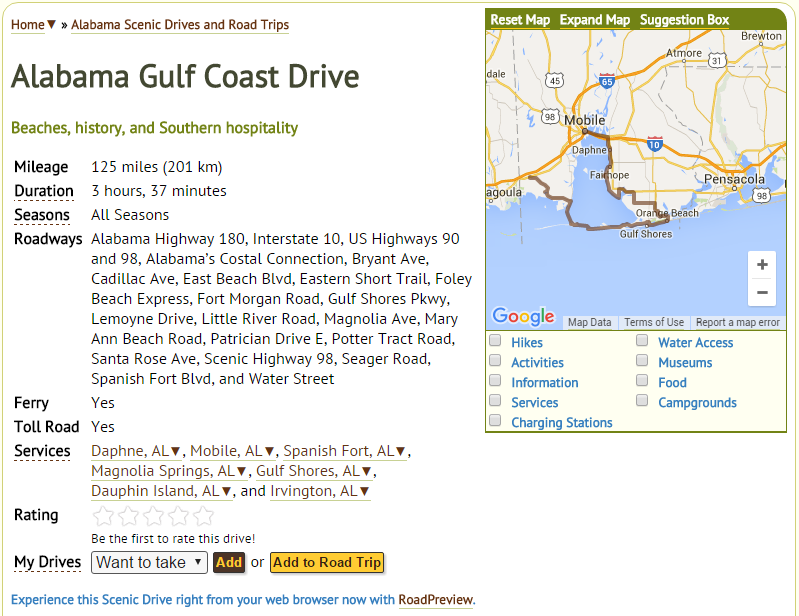
\includegraphics[width=0.45\textwidth]{images/background/msd_rdp.png}
	\end{center}
	\vspace{-6mm}
	\caption{MyScenicDrive's route details}	
	\vspace{-10mm}
\end{wrapfigure}
MyScenicDrives is a website that allows users to search for scenic routes by city, state or zip code (currently the service is only available in the United States), and view extremely detailed information about these routes. This includes a very lengthy explanation of all the things can be seen and done on the journey, interesting facts about the locations visited, all the roads that will be driven on, the best seasons to take the journey during, and even which service stations will be passed. This extremely rich content is the main selling of MyScenicDrives.

\vspace{5mm}
\noindent 
However, no matter how high the quality of this content it, there is still a glaring problem with MyScenicDrives: the quantity of routes. This may be due to the huge amount of information required for a route to be accepted onto the site, but essentially makes the entire application useless. As an example, a search for all routes in the state of Alabama returned a single result. In addition to this, the search functionality itself is very primitive. There is no option for users to select where they wish to start or end their journey, and instead they can only pick a large geographic region. Which would not be suitable for Niceway.to, which aims to provide a way for users to find routes between specific locations.
\ \\
\paragraph{Mad Maps, \url{http://madmaps.net/}}\ \\
The final mapping website that was investigated was Mad Maps, which differed from the others in that it allowed users to purchase physical maps, which they could also view on their mobile phones. One useful feature of the service was the ability to download routes directly to a mobile device, so that the user's Internet connection did not become a limiting factor during a journey. However, it is difficult to ignore the biggest down fall of this service, which was the cost associated with it. All of the maps had a price associated with them, and there was no ability to preview the maps before purchasing. This blind investment could be off putting for many users, as they may be unsure if they will even enjoy the routes provided. Further to this, the mobile application both required an upfront payment to download, as well as containing adverts within it: which seems unjustified when the majority of the Mad Maps applications had very poor reviews.
\begin{wrapfigure}{l}{0.4\textwidth}
	\vspace{-1mm}
	\hspace{5mm}
	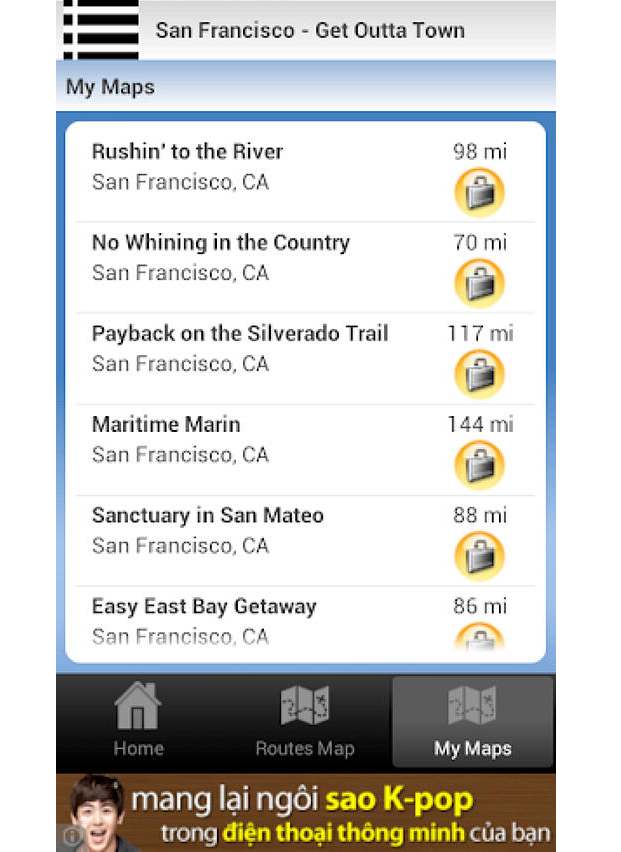
\includegraphics[width=0.35\textwidth]{images/background/mm_rlp.png}
	\centering
	\caption{List of Mad Maps routes}	
	\vspace{-40mm}
\end{wrapfigure}
\ \\
The service works by having a group of ``experts'' compile the maps, and distribute them to the users. This is supposed to instil confidence of their quality, but instead takes out a huge part of travelling, which is the social experience. The only social interaction that users can have with Mad Maps, is the ability to upload photos of waypoints that they have visited, but these will then only be seen by other users that have purchased the route, and would not help to foster the community that Niceway.to is striving for. 

\newpage 
\subsection{Platforms and Tools}
\label{sec:pat}
This section introduces some potential platforms and tools that could have been used in the project, along with justifications for and against them. The system consisted of the back end and server technologies, as well as some user-friendly front end. Tools and frameworks and languages for both of these parts were evaluated to determine which would be the most appropriate. A full list of the final decisions of tools to use, including their justifications, can be found in section \ref{sec:kid}.

\subsubsection{Native Mobile Applications VS Responsive Web Applications}
Before investigating technologies to use, it was important to determine what kind of application was to be developed, as this would radically change the tools required. Ultimately, it was decided that it would be better to build Niceway.to as a responsive web-application, but the advantages and disadvantages of both approaches have been discussed below.

\paragraph{Native Mobile Application}\ \\
Native mobile applications are applications that are downloaded onto a mobile device, and run directly on the hardware. These applications generally have greater exposure, because they are distributed through the application marketplace for the given operating system, and can be reviewed and rated by users. There are several advantages to developing a native mobile application including: the ability to implement multiple pricing models (payment for download, in-application purchases, free with advertisements, or entirely free), after the initial download they can be used without an Internet connection (as data can be downloaded to the phone and accessed later), and the native technology and hardware of the phone can be utilised to provide a better experience for the user.\ \\
\ \\
However, native applications do also have some drawbacks. The most prominent is the number of different operating systems available, which mean that any application created needs to be rewritten multiple times in different languages, to ensure that it can target all devices. This is a huge investment of time and resources, especially as some platforms do not have a large user base (and therefore this effort would potentially be wasted). Native applications must also be downloaded onto the user's device, which requires a commitment from the user, and their on-going desire to keep the application on their phone. Mobile phone users can be fickle, and delete the application at any time for any number of reasons. 

\paragraph{Responsive Web Application}\ \\
A responsive web application is a website that can function both on desktop devices, and mobile devices by scaling the elements on display. They are incredibly versatile because they run in a web browser, which means that they target all possible devices without the need to rewrite the code base in several languages (some tweaks for certain browsers may be required, but this is usually a small amount of work). They are written in the default web languages of HTML, CSS and JavaScript, and the back end can be whichever language the developers are most comfortable with, which makes it very easy for developers of any skill level to work on them. Another advantage of them being hosted on a server online is that it becomes very easy to release updates, because they are instantaneous, and the users do not have to download anything.\\
\ \\
However, the Internet is a large place, and without a centralised place to advertise the application, it is possible it will never be discovered by many potential users. Alongside this, web applications require a constant Internet connection to access them, which could be a problem for users that do not have a large data allowance on their phone.


\newpage 
\subsubsection{Back End Tools}
{\color{purple}
Language  - framework pairs
}

\paragraph{The Zend Framework (PHP)}\ \\
{\color{red} What is it, why it's good, why it's not}

\paragraph{Ruby on Rails?}\ \\
{\color{red} What is it, why it's good, why it's not}

\paragraph{Javascript with Node.js}\ \\
{\color{red} What is it, why it's good, why it's not - good because all one language!}


\subsubsection{Front End Tools}
{\color{purple}
After it was decided that it was to be a web app, the language choice was obvious, so I looked at front-end design frameowkrs instead instead.
}
\paragraph{Bootstrap}\ \\
{\color{red} What is it, why it's good, why it's not}

\paragraph{Foundation}\ \\
{\color{red} What is it, why it's good, why it's not}

\paragraph{Semantic}\ \\
{\color{red} What is it, why it's good, why it's not}
\newpage 
\section{System Specification}
\label{sec:spec}
In this section, the functional and non-functional requirements of the system have been outlined. These were obtained by looking through the design specification that the client provided at the start of the project, and were agreed upon by both parties. 

\subsection{Functional Requirements}
\label{sec:funcs}

 \begin{enumerate}
 \item[1.] The user should be able to search by geographic region and discover submitted routes for that region.
 \item[2.] The user should be able to contribute routes.
 	\begin{enumerate}
 	\item[2.1.] Only the creating user should be able to modify these routes
 	\item[2.2.] The user should be able to decide on the visibility of this route
 	\end{enumerate}
 \item[3.] The user should be able to interact socially with the route, including:
 	\begin{enumerate}
 	\item[3.1.] Comment on public routes
 	\item[3.2.] Recommend alternative routes
 	\item[3.3.] Share routes to external social media websites
 	\end{enumerate}
 \item[4.] Users should be able to create an account with, for example, name, email and location 
 \item[5.] There should be administrative users who have extra functionality, including:
	 \begin{enumerate}
 		\item[5.1.] Managing users
 		\begin{enumerate}
 			\item[5.1.1.] Delete users
 			\item[5.1.2.] Update users
 			\item[5.1.3.] Create users
 		\end{enumerate}
 		\item[5.2.] Managing routes
 		\begin{enumerate}
 			\item[5.2.1.] Delete routes
 			\item[5.2.2.] Update routes
 		\end{enumerate}
 		\item[5.3.] Delete comments
 		\item[5.4.] Make announcements
 		\item[5.5.] Make backups of the website in a standard, compliant, free and open format
 		\item[5.6.] De-authorize active sessions
 		\item[5.7.] Lock the site and prevent access
 	\end{enumerate}
 \item[6.] Users should be able to export their routes to a FOSS
 \item[7.] Users should be able to make a copy of other user's public routes and edit them
 \item[8.] There should be a route editor component which allows the users to specify a route
 \item[9.] The user should be able to log into their account and:
	 \begin{enumerate}
	 	\item[9.1.] Access and change personal information
	  	\item[9.2.] Access and edit their submitted routes
	 \end{enumerate}
 \end{enumerate}

\paragraph{Accessibility}\ \\
The proposed system is to be made available entirely on-line, allowing anyone with internet access, and a computer, to use the system. As the application will be web-based, the user is not required to download anything to start using it, which will make it more accessible for the user, and easier for them to get started using the application. The only potential issue with a web-based application is if the server goes down, or if the domain expires. The server going down does not, unfortunately, have a solution, but keeping the domain should be relatively trivial.

\paragraph{Usability and Operability}\ \\
The project should be designed in such a way that users ranging from a low level of skill, to a high level of skill should be able to use it with little prior knowledge. Help will be available within the system, so the user can received help and directions, without having to leave the system and check some external documentation. The project will be developed as a fully-responsive web application, meaning mobile devices will be fully supported.

\paragraph{Maintainability \& Documentation}\ \\
The system must be exceptionally well documented allowing for easy maintenance by an external developer. This includes both an easy to understand code structure, as well as commented code (specifically using PHPDoc, and a similar style in the JavaScript code), which should be kept as modular as possible.  The system itself will have help available to the user, so that if they are confused, they can be guided in the right direction.

\paragraph{Quality}\ \\
As this system is to be used externally, and will be a representation of both myself, and the client, there are several quality issues that must be addressed. The system must be built so that it is robust, and works as the user expects, but it must also contain as few bugs as possible. Any bugs that are identified should be reportable to the maintainer, and be fixed as soon as possible.\ \\
\ \\
The quality of the code must also be considered. In this regard, the code will be written in a modular way, and useful comments will be provided to highlight the purpose of each function, and to illustrate any particularly complex code.

\paragraph{Resource Requirements and Constraints}\ \\
As this system is aimed at users with a mixture of skill levels, no assumptions can be made on the level of hardware that the users will possess. For this reason, the system will be designed to use as few resources as possible. Fortunately, due to being a web-based system, the load of the system would be fairly minimal anyway, as it is mostly loading only JavaScript and HTML5. The only true computation takes place on the server, and thus would not be a concern for the user.\ \\
\ \\
The ability to load and save files potentially causes a problem, but only if the user has very little hard drive space, and attempts to save an extremely large file from the system. Unfortunately, there is nothing that can be done about this, but even very large systems will have a relatively small file size.\ \\
\ \\
The final concern is internet bandwidth which, whilst not a problem on desktops, will be a problem for mobile phones. This is why the amount of data sent to the user when they are navigating a route will be kept to a minimum, so that they do not use up their data allowance (or drain their battery).

\paragraph{Cross Platform Compatibility}\ \\
Due to the project being a web-based system (developed using HTML5, CSS3, and JavaScript), it is difficult for it not to be cross platform compatible. However, there are still a few issues that may have to be dealt with, especially when looking at different browsers that the user may be using. For this reason, research into how the system performs on different browsers will be important, so that it can be assured that any user using any browser will have full access to the system, as it was meant to be.

\paragraph{Security}\ \\
Security is a concern for this project, as the users will be able to create accounts with the system, and therefore their data will need to be stored. This data will be stored in compliance with the Data Protection Act, and all passwords will be encrypted. 

\paragraph{Disaster Recovery}\ \\
The administrator should be able to take backups of the site in a standard, compliant, free and open format. They should also be able to de-authorize active sessions, and lock the website to prevent access. As far as the code base itself, the project will be stored both on the server, and in a Git repository, allowing for recovery if anything goes wrong.
\newpage 
\section{System Designs}
In this section, all of the design aspects of the system have been detailed and justified. This includes the design of the user interface itself, the navigation and expected user path, and the internal design of the application.

\subsection{Navigation/Control Flow Design}
In the final implementation of the system, there were seven main sections, which have been enumerated below with a brief explanation of what their main purpose is.

\begin{enumerate}
	\item Route Discovery \ \\
	The landing page, which provides a large search box (allowing users to search for routes), and a description of the main functionality of the website.
	\item Route Listing \ \\
	The search results page, which would list all of the results returned for a particular set of search terms, as well as some brief information about each of the routes.
	\item Route Detail\ \\
	The individual route display page, which lists all the available information for a given route, as well as the social stream that users can interact with.
	\item Route Creation\ \\
	The map interface that allows users to specify their own routes, as well as an interface for listing the points on the route.
	\item Profile Page\ \\
	The user detail page, which allows registered users to view their own routes and their saved routes, edit their settings, and update the appearance of their avatar.
	\item Admin Page\ \\
	The administrator only page which gives them access to various administrative tools, as well as the ability to look at and handle reported content.
	\item Login/Signup Pages\ \\
	Pages that provided short forms allowing users to either sign up or log in to the system.
\end{enumerate}
\noindent 
When designing a website, it's important to think about how the users of that website will traverse it, depending on their goals. For Niceway.to, there are two main user groups to consider: those with accounts, and those without accounts. Both of these groups will use the site in very different ways: those users without accounts will use the site simply for the searching of routes, but those \emph{with} accounts will be much more involved in the social aspects of the site and sharing their own content.\ \\
\ \\
The path that users \emph{without} accounts would usually take, as shown in figure \ref{fig:nonuser_flow}, would start with the landing page. They would then follow a rather linear path through the system, as they are only given the choice to advance to the next page in the sequence (or back if they so wish). This starts with searching for a route, selecting a route from the search results, viewing the detail page for this route, and then potentially looking at the route in ``full-view'' (where we see the route displayed in a map filling the entire screen). At any point in this sequence, the user is free to jump to the sign up page, a link to which is located in the top right hand corner of every page.

\begin{figure}[!ht]
	\begin{center}
		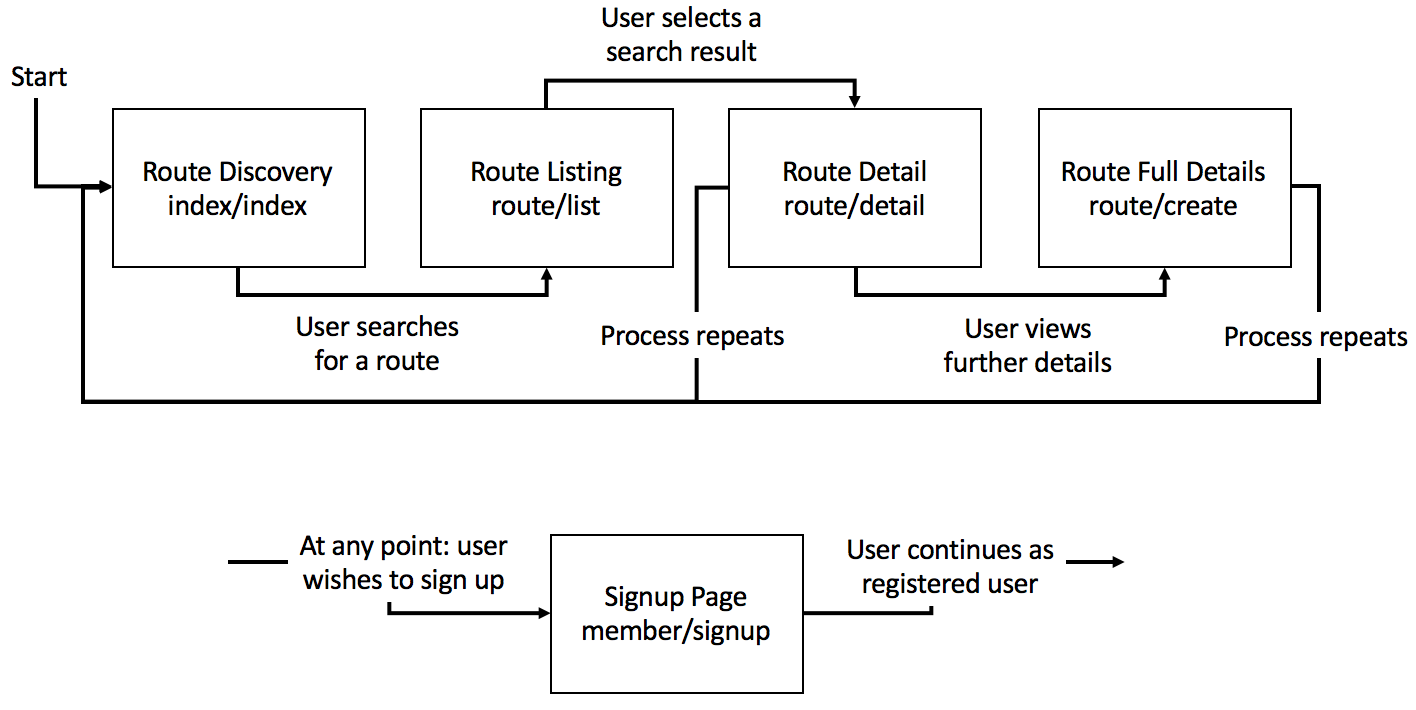
\includegraphics[width=0.9\textwidth]{images/design/nonuser_flow.png}
	\end{center}
	\vspace{-6mm}
	\caption{Expected path of non-registered users}
	\label{fig:nonuser_flow}
	\vspace{-5mm}
\end{figure}

\noindent 
For a registered user, we can expect a much less linear path, due to the larger quantity of actions they have available to them, this path is shown in figure \ref{fig:user_flow}. Unlike the non-registered users, there's no requirement for these users to start on the landing page, as it can be assumed that they would have book marked specific pages, and would log in to access them. After logging in, it is expected the user would spend some time on their profile page, and then use this page as the springboard to one of three main available actions: looking at their own routes or routes they are interested in, creating a new route, or following the same route search flow as non-users would.

\begin{figure}[!ht]
	\vspace{-3mm}
	\begin{center}
		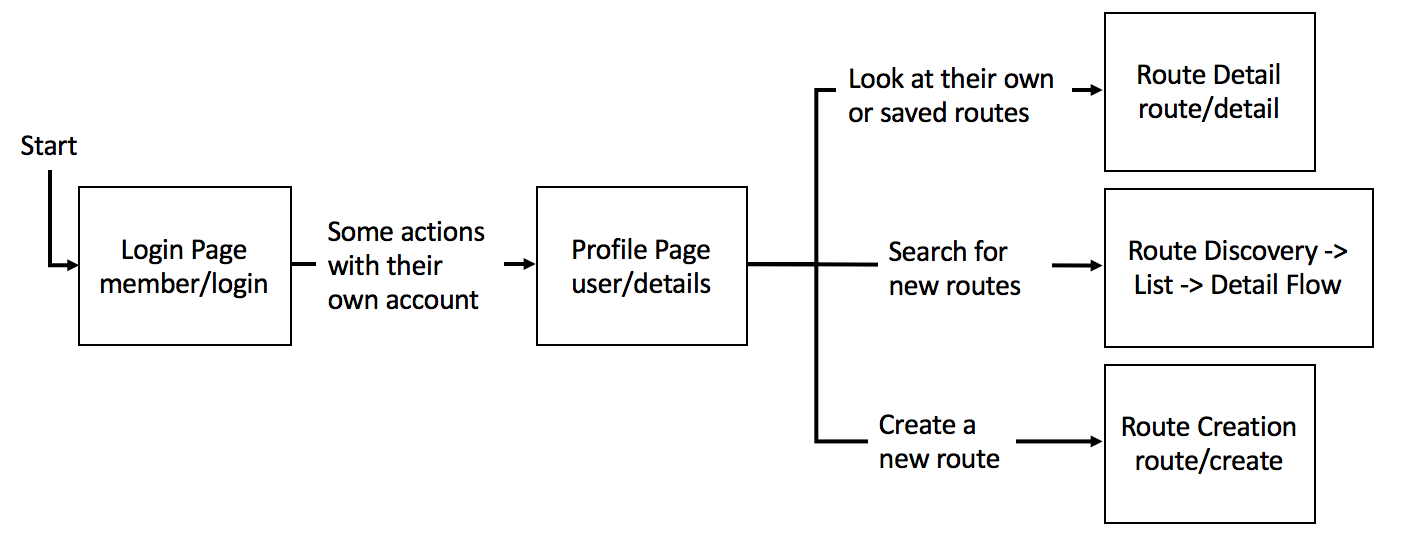
\includegraphics[width=0.9\textwidth]{images/design/user_flow.png}
	\end{center}
	\vspace{-6mm}
	\caption{Expected path of registered users}
	\label{fig:user_flow}
\end{figure}

\noindent
Of course, this is just the generally expected path, and users are in no way restricted to what they can do (with the exception of accessing the search results page without having performed a search). The user can access any page of the site from any other page, through use of the navigation bar present on every page (shown in figure \ref{fig:navbar}), which provides links to the search, creation, profile, and administrator sections of the website. This navigation helps to promote freedom and a sense of control within the system. This means that even when users make mistakes, they should feel like they know how to go back and rectify these mistakes, rather than being stuck in a state they do not wish to be in.

\begin{figure}[!ht]
	\begin{center}
		
\includegraphics[width=0.9\textwidth]{images/design/navbar.png}
	\end{center}
	\vspace{-6mm}
	\caption{The navigation bar displayed to registered users}
	\label{fig:navbar}
\end{figure}

\subsection{User Interface Design}
In this section, the interfaces for each of the main pages of the application have been displayed, along with justifications for why they were designed the way they were. Designs for each of these pages were produced at the beginning of the project and shared with the client. The design presents here are based on his feedback, and a combination of the best features from all the other designs. The initial designs can be found in appendix \ref{sec:isd}.

\paragraph{Route Discovery Page/Landing Page}\ \\

\begin{figure}[!ht]
	\vspace{-6mm}
	\begin{center}
		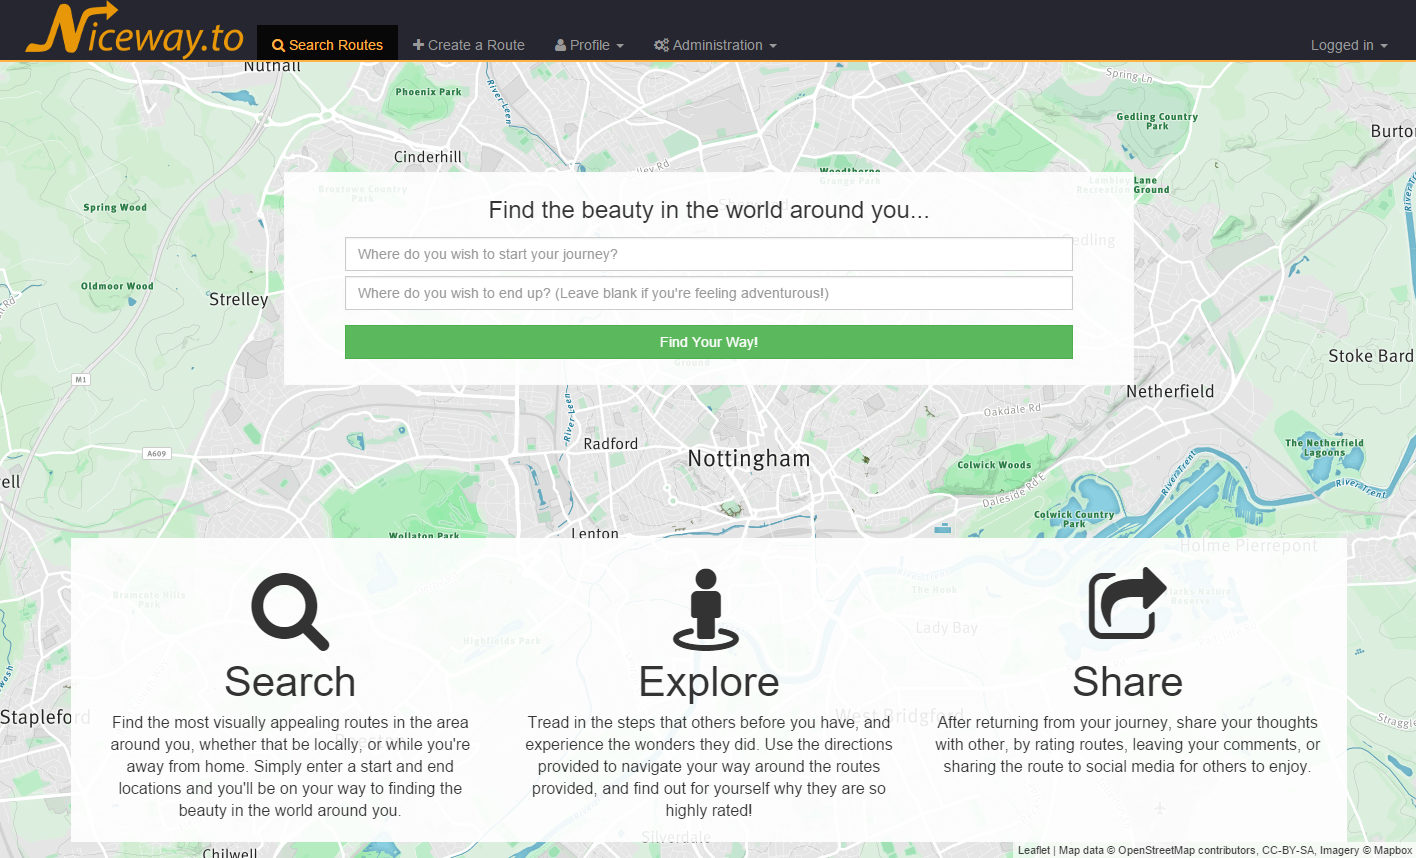
\includegraphics[width=0.95\textwidth]{images/design/landing.png}
	\end{center}
	\vspace{-7mm}
\end{figure}
\noindent 
The design of the landing page was as simple as possible, with a large search box in the centre of the page (similar to Google), and a small infographic describing the purpose of the website. The prominent search box promotes the main functionality of the website, and makes it extremely easy for users to get started on their journey, without them being distracted by superfluous extra details. The page aims to look attractive to the user, so they are more compelled to use the site, rather than being put off, and taking their interest elsewhere.

\paragraph{Route Listing Page}\ \\

\begin{figure}[!ht]
	\vspace{-5mm}
	\begin{center}
		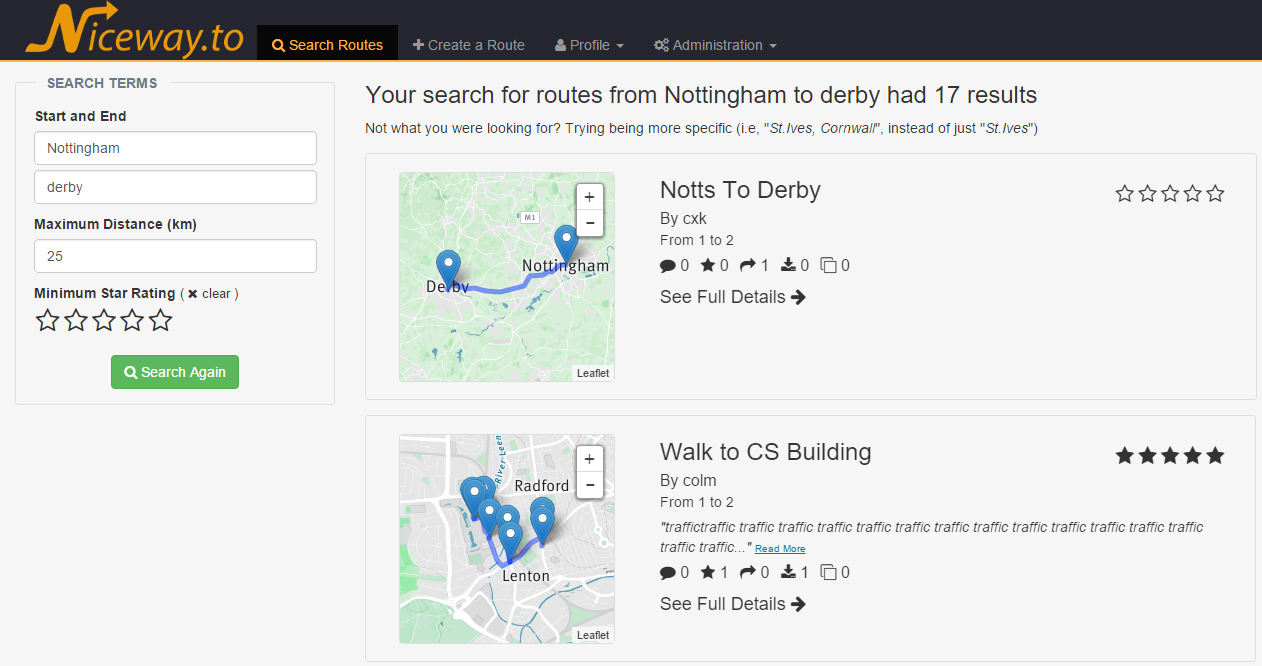
\includegraphics[width=0.95\textwidth]{images/design/listing.png}
	\end{center}
	\vspace{-10mm}
\end{figure}
\newpage 


\noindent 
The route listing page was used to describe the key details of the routes that matched the user's search terms. During the design stage, two main approaches were considered: displaying the routes on a map, or displaying them individually. The problem with the former approach would be when there were a large number of results returned, which would cause the map to look cluttered, and it would be difficult for users to distinguish between routes. The listing approach allows each route to be considered individually, as well as being put in some kind of order (which is where the rating system is utilised). \ \\
\ \\
A form on the left hand side (as well as the large title next to it) is present so that users can see the terms they searched for, and make any amendments necessary if there were mistakes (it is placed on the left because western cultures are more likely to look at the top left of a page first\cite{mccarthy2004could}, which allows users to identify their errors earlier). It also allows them to further refine their search, with a minimum star rating, and maximum distance from the entered points. The key points of each route are displayed on this page, so users can make a decision as to which ones they which to investigate further. This includes the name and description, as well as social ranking, such as the rating and number of social interactions made on that route. The idea being that a user should very quickly be able to decide if a route is worth visiting or not, so they do not find they are wasting their time looking at poor quality routes.

\paragraph{Route Detail Page}\ \\
\begin{figure}[!ht]
	\vspace{-6mm}
	\begin{center}
		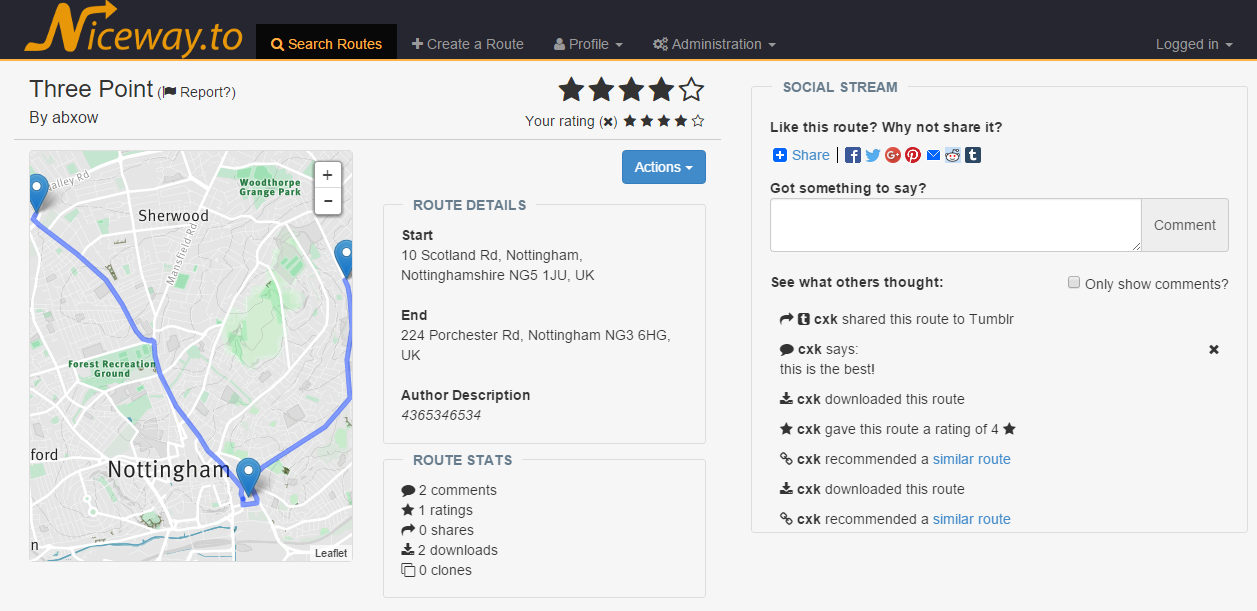
\includegraphics[width=0.9\textwidth]{images/design/detail.png}
	\end{center}
	\vspace{-8mm}
\end{figure}

\noindent
The route detail page was the page used to list all information about one specific route - for this reason, there was a lot of potential for this page to become cluttered. To combat this, the page is clearly divided into two main segments, which are then also further divided. These main sections were the route details on the left, and the route social stream on the right. This clear separation and hierarchical structure to the page made it very easy for users to locate specific information, by slowly narrowing down their search to different areas of the page. \ \\
\ \\
The details section of the page contained a map of the route, key information about it (both administrative information like its name, and practical information like where it starts), as well as social statistics, like the number of comments and shares (allowing users to see a numeric representation of the popularity of the routes). This meant that users could garner all the information they needed to actually experience the route, as well as see the route they would be following. Being on the left, it is likely users will look at this section first, which means they can quickly determine if they have navigated to the wrong route.\ \\
\ \\
On the right was the social stream, which displayed an amalgamation of all user social interaction with the route. This included comments, shares, downloads, and all other social interactions available. The purpose of this was to give a complete picture of the all interaction with the route, so that users could fully immerse themselves in it, and see what the community thought. It is very prominently displayed, so that more users are likely to notice it, and are more likely to interact with it (a point that my client stressed was extremely important). The social stream was visible both to users that were logged in, and those that weren't. This meant that registered users could easily share their opinions and interact with the route, and non registered users were more convinced to register, so they can could join in with the discussion.

\paragraph{Route Creation Page}\ \\
\begin{figure}[!ht]
	\vspace{-5mm}
	\begin{center}
		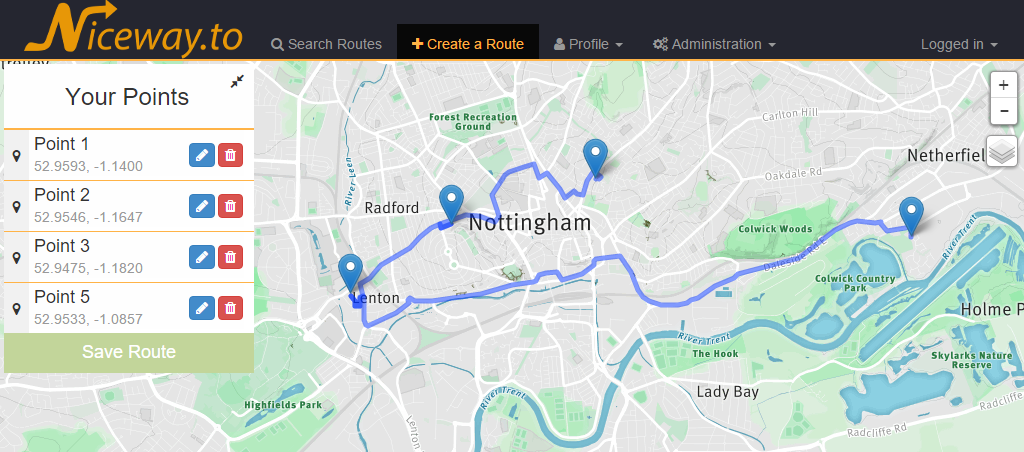
\includegraphics[width=0.99\textwidth]{images/design/create.png}
	\end{center}
	\vspace{-5mm}
\end{figure}

\noindent 
The route creation page was the page that would be used to actually construct and edit routes. It has a very simple interface that consists of a large map and a list of points on that map. This meant that the user could focus on the primary objective of the page, which was the creation of their route, without being distracted by other, useless interface elements. The list on the left served as a tool for users to track what they had done, easily jump to specific points, and update them. This list could also be collapsed, to take up even less space, to further reduce clutter and allow users to see their maps unobscured.\ \\
\ \\
To add points, users only had to click on the map, which meant that using the page was very simple and intuitive. As points are added to the map, a route is drawn between them, during which time a popup is displayed so the user is aware of this. The advantage of drawing the map after each point, is that the user can see how their route is forming, and can make adjustments on the fly, rather than getting to the end, generating the route and realising they'd made a huge mistake. \ \\
\ \\
When the user is done with their route, they can click the save button to bring up a modal window, allowing them to enter in the name and description of the route. Having this in a modal window helps to further eliminate clutter on the page, as it is only displayed when the user specifically requests it.

\newpage 
\paragraph{Profile Page}\ \\

\begin{figure}[!ht]
	\vspace{-5mm}
	\begin{center}
		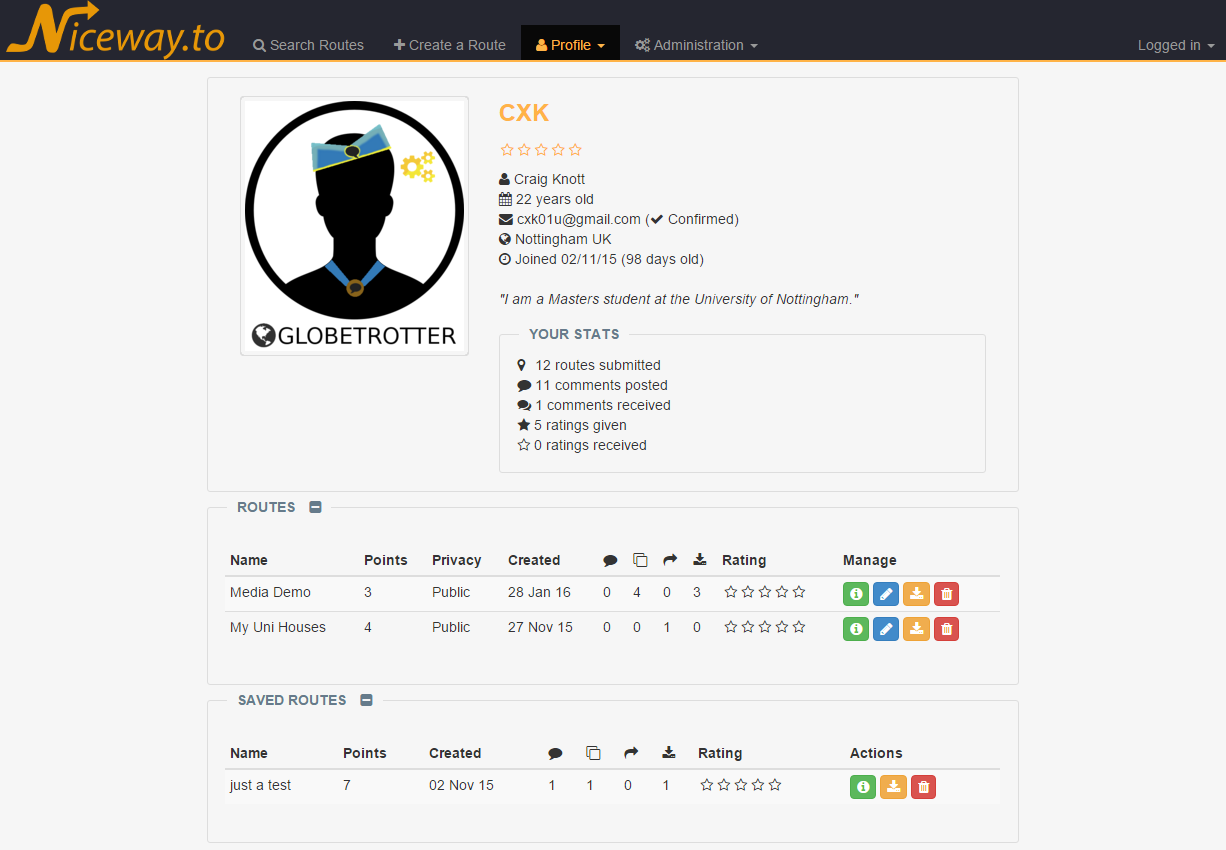
\includegraphics[width=0.95\textwidth]{images/design/profile.png}
	\end{center}
	\vspace{-5mm}
\end{figure}
\noindent 
The final major page of the website is the user profile page, which displays information about a specific user, a list of their routes, and a list of their saved routes. The purpose of this page was to allow users to express themselves to other members of the community, and have somewhere to call ``home''. It displays their public and private details, like their customisable profile image, email, account age, and location, as well as statistical information, like the number of comments their routes have received. This meant that other users could quickly build up an idea of what this user is like, and how they interact with the application.\ \\
\ \\
This page also displayed all of the routes that the user had created, which served a different purpose depending on whether you were viewing your own account page or another user. If viewing your own account page, it served as a central hub to administer and manage all the routes that you had produced, by listing them all, and providing functionality to view them, edit them, or delete them. If viewing another user's profile all of their public routes would be on show. From here, users can view, clone, or download the routes, but not actually make any changes to them. This meant that users could look at the profile of a content producer they enjoyed the work of, and look at other work they had produced. 


\subsubsection{Heuristic Evaluation of the Interface}
In this section, the user interface is evaluated using several key metrics. These include the general purpose usability heuristics identified by Jakob Nielsen\cite{nielsen199510}, and the golden rules of interface design identified by Ben Schneiderman\cite{shneiderman2005designing}. These have been grouped together, with the specific heuristics being labelled in brackets (JN for Jakob, and BS for Ben), a full listing of all the heuristics referenced in this section can be found in appendix \ref{sec:idh}.

\newpage 
\paragraph{Visibility and Feedback (JN1, BS3)}\ \\
Users should always be aware of the impact of their actions. This is why any user interaction will have some visible feedback to the user, which will usually either be the updating of the interface (if something is added or removed), or popup modal windows informing users of what has happened, or what is about to happen.

\paragraph{User should be in full control (JN3, JN7, BS4, BS7, BS8)}\ \\
Users should always be in charge of their experience of the website. This is why they are given full freedom to navigate anywhere within the system (using the navigation bar), and to decide what actions they wish to perform. At no point is the user forced to do anything they have not explicitly requested.

\paragraph{Consistency (JN4, BS1)}\ \\
Consistency is important within a system so users can become accustomed to how things work, and what they mean. This is especially important when users are accessing new features for the first time, because they can use their previous knowledge to help them understand the new functionality. This is why colours and icons will be used heavily throughout Niceway.to. Green colours will be used to resemble positive actions (like adding or accepting), and red will be used for negative (deleting or cancelling). Icons for different aspects of the system (like cloning routes, or downloading routes) will be implemented and kept consistent so that users will associate specific icons with specific actions, and they will easily be able to locate and achieve their goals.

\paragraph{Error prevention and Recovery (JN5, JN9, BS5, BS6)}\ \\
It is important that users do not feel punished for making mistakes, and do not get trapped in error states, unable to return. For this reason, extensive error prevention will be implemented, including validation on all forms, confirmations on ``dangerous'' actions, and useful error messages being provided when mistakes are made. The language of these messages is extremely important, as to not make the user feel like they have done something wrong. Instead, users should be instructed on how to resolve the problems they have encountered.

\paragraph{Reduce Cognitive Load (JN6, JN10, BS8)}\ \\
A simplistic design is vital, otherwise users will be encumbered by the sheer quantity of content (it has been shown that humans can only truly cope with between 5 and 9 things at a time\cite{miller1956magical}). If there is too much on the screen at once, users will be confused and unable to focus. This is why only relevant and useful data will be displayed to the user, and interfaces will be as minimalistic as possible. Another way to reduce the cognitive load on the user is to remember data for them. This principle will be applied on the search results page, where the search terms are displayed back to the user, allowing them to be dropped from the user's short term memory. 

\paragraph{Match between system and the real world (JN2)}\ \\
The system should use language and imagery that is common and well known, rather than specific to the application. This helps the user's general understanding of the system, as they can relate it to other systems they have used. One example of this in practice is the use of the word ``clone'', for the forking of routes. Forking is a term well known in the field of computer science, but many average users would not understand it, hence this simplification. This is also the reason that icons are used throughout the system, as many users will recognise them and will understand the system better with their inclusion.

\newpage 
\subsection{Internal Design}
As well as the front end, the inner workings of the back end of the system also needed some design. At this point during the project, the Zend framework had been picked as the back end framework (for reasons discussed in section \ref{sec:kid}), which enforces a Model-View-Controller design pattern. The advantages of the MVC framework are that it is simple to understand and use, provides separation of the accessing, processing and display of data, and is extremely modular. The diagram in figure \ref{fig:mvc} shows the interaction that users would have with the front end and back end of the system. It begins with a user on some web-browser making a request for a specific page. The browser then talks to the Controller (firstly the base controller, and then the specific controller for that page), which usually requests some data from the database. This access is abstracted, and is facilitated through the Model and various factories of the system, which actually access the data, and returns the results as a PHP object. The controller then passes this data on the View, which displays the user interface and is served to the client for them to interact with.

\begin{figure}[!ht]
	\begin{center}
		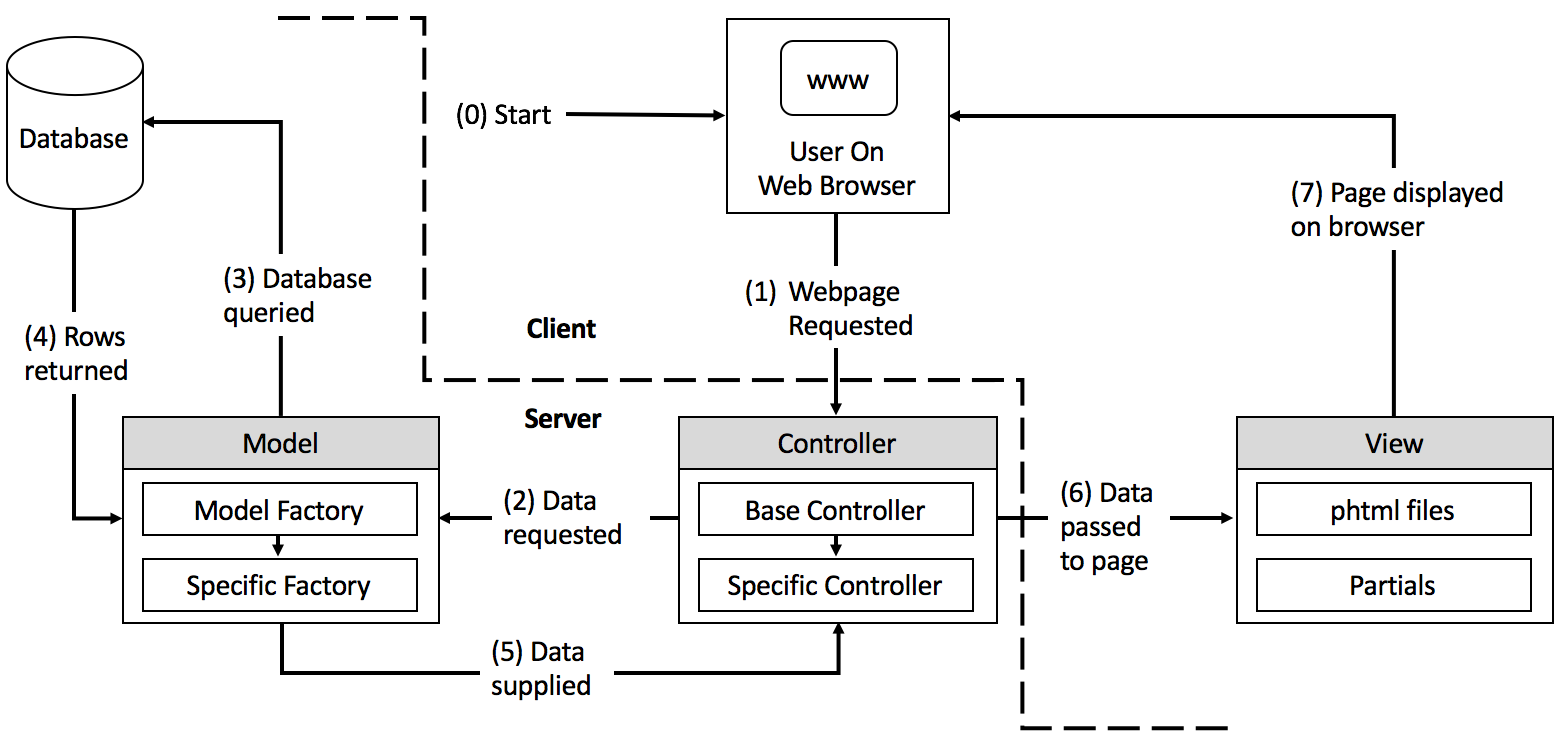
\includegraphics[width=0.9\textwidth]{images/design/internal.png}
	\end{center}
	\vspace{-6mm}
	\caption{The internal design of Niceway.to}
	\label{fig:mvc}
\end{figure}


\newpage 
\section{Software Implementation}
In this section, the actual implementation of the software has been detailed, including: what tools were used in the implementation, how the software was implemented, and any issues that were encountered during the implementation process.

{\color{red}
	\begin{itemize}
		\item Screenshots of initial designs + justifications
		\item Screenshots of final designs + justifications + reasons for changes
		\item Screenshots of actual final system + reasons for changes
	\end{itemize}
}

\subsection{Key Implementation Decisions}
\label{sec:kid}
{\color{red}
	\begin{itemize}
		\item From the background research section, list all the technology I chose to use and why
	\end{itemize}
}

\subsection{Implementation Methodology}
{\color{red}
	\begin{itemize}
		\item To help manage the implementation of such a large piece of software, the adoption of some methodology was necessary. It was decided that the best methodology would be an agile one, with heavy use of Kanban, using the tips laid out by Henrik Kniberg \cite{kniberg2007scrum}. In order to accomplish this, at the beginning of the implementation stage, after the requirements specification had been detailed, the entire project was split into user stories. Each of these stories detailed a specific action that a user of the system would be able to accomplish, along with how long it should take to implement, how important it was, and a way of testing its completion. These stories were then organised onto a digital Kanban Board, using a service called Trello\footnote{\url{http://www.trello.com}}. \ \\
		\ \\
		Each week, a set of tasks would be selected to be worked on for that week. The amount of tasks selected would be dependent on how much was completed, on average, in the weeks before, so that reasonable estimates could be made (obviously excluding the first few weeks). This ensured a decent portion of work was being completed per week, and that progress was constant. During the week, tasks would be selected from the available pool, prioritising those that were prerequisites of others, or had a high importance, and would then be worked on until completion. After the completion of a task, a new task would be selected, and work would begin on this. This was an extremely effective method of managing the implementation, as any small tasks that were necessary could be added to the board, and there was an assurance they would eventually be completed, and nothing would be overlooked. It has also been shown that it is much easier to reach goals if they have been written down \cite{wilson2008goal}, which a Kanban Board was the perfect tool for.\ \\
		\ \\
		Also mention weekly meetings with max and use of Gantt chart. Also mention this is what I did at work and in my last diss and found it the best way to work for me?
	\end{itemize}

}
{\color{blue}
	full example of taking a requirement, making story, splitting into sub tasks (in table or screenshot format)
}

\subsection{Implementation of System Components}
{\color{red}
	\begin{itemize}
		\item Potentially don't need this
		\item Do last, look at last year's diss
	\end{itemize}
}


\subsection{Problems Encountered}
{\color{red}
	\begin{itemize}
		\item Look through problem log document and pick out key things, especially those with lessons
		\item What happened / what this affected / how the project was affected / what I would do differently / why it happened
		\item problem: lack of unit tests meant that the addition of features would break others. especially silly with the support Zend has for unit tests
	\end{itemize}
}
\newpage 
\section{Evaluation of the Project}
Testing and evaluation were vital parts of the project, to ensure that the system contained all the functionality it should have, adhered to all the constraints place upon it and that it was actually usable. Three stages of testing were therefore conducted. The first of these was functionality testing, in which the functional requirements of the system would be evaluated, and the system would be tested to see whether or not it implemented this functionality. The next stage was non-functional testing, in which the non-functional requirements would be evaluated, to ensure the system abided by them. The final stage was user feedback testing, in which a group of participants would actually be using the system. In this stage, three systems would be evaluated: MATLAB, FuzzyToolkitUoN, and this project; in order to determine which provided a better user experience.

\subsection{Functional Testing}
In this section, each of the functional requirements laid out in section \ref{sec:funcs} have been evaluated in turn, to ensure the system meets them. Knowledge of the inner workings of the system is not actually necessary to understand these tests, as they simply check whether functionality is present, and are not concerned as to how the system actually implements it (this is known as black box testing \cite{beizer1995black}). A complete listing of all the tests conducted, and their results, can be found in appendix \ref{app-ctl}.

\subsection{Non-Functional Testing}
In this section, each of the non-functional requirements laid out in section \ref{sec:non-funcs} have been enumerated, and the success to which they have been achieved has been detailed. The purpose of this is to evaluate how well the system has adhered to the constraints placed upon it.

\paragraph{Accessibility}\ \\
This was one of the biggest goals for the system, as it was one of it's main reasons for conception. The problem with most fuzzy logic software systems currently is that they are difficult to use, or difficult to access. That is why the project proposed in this report has accessibility improvements as one of it's main goals. To accomplish this, the system is entirely web based. The advantage of this, is that the user can access the system from any computer, running any operating system. This cross compatibility greatly improves the outreach of the software, as no users will be unable to access it. Further to this, the system front end is constructed entirely in HTML, CSS, and JavaScript. This means that the user does not require the download of any additional software, or applications, to use this system (which would not be case if Adobe Flash, or Java had been used). 

\paragraph{Usability and Operability}\ \\
This is a goal of the system that is difficult to quantitatively measure. In order to actually test this goal, a set of participants of varying skill levels were asked to complete a list of tasks, using this system, and compare this to doing the same tasks in similar systems. The detailed results of these tests can be found in section \ref{sec:uft}. After the user feedback testing, it was found that the majority of participants preferred this new system, over the other two that were tested (MATLAB's fuzzy toolbox, and FuzzyToolkitUoN). The major reasons for this were the ``waterfall'' style to task completion (each task was laid out in a logical manner, and followed on smoothly from the last), and the clean, uncluttered user interface. 

\newpage
\paragraph{Maintainability}\ \\
To aid with the eventual goal of the system back end being interchangeable with any back end that can process fuzzy logic, the system needed to be coded so that it was easily maintainable, and easily expandable. In order to achieve this, the code has been written in a modular fashion, split across multiple files. Each file deals with exactly one action (file manipulation, rule creation, evaluation, etc.), and thus adding new functionality should be relatively easy. Each function has been listed with the purpose of it, the parameters it takes (and their types), and the value it returns, if any. This means identifying the purpose of functions is extremely simple, and any maintainer will easily be able to interpret how the system works. 

\paragraph{Quality}\ \\
To ensure that this system reflects well both on myself, and the University of Nottingham, it was made to be of the highest quality possible. The system has been built with a vast quantity of error handling methods, so that the system should not crash under operation, and should function exactly as the user expects. Helpful, and positive, error messages accompany any error handling methods, so the user can rectify any mistakes they make (without feeling punished for making them). 

\paragraph{Resource Requirements and Constraints}\ \\
As the system is aimed at any level of user, no assumptions as to the level of hardware they may possess can be made. This means that the system must be built to be as light weight as possible, as to not overwhelm the user's device. Fortunately, the technologies used to build the front end (CSS, HTML and JavaScript) are relatively light weight, and the front end has minimal processing requirements. The main processing that takes place is on the server side, when inference occurs.

\paragraph{Cross Platform Compatibility}\ \\
As mentioned previously, the system is built with entirely cross compatible languages, and only requires the user have an internet connection, and a web browser installed to be accessed and used. Aside from these, there are no compatibility issues the system presents, as it is entirely web based, and requires no additional resources to function. There is potential that the system would not work on extremely old operating systems, but all operating systems that are currently being supported by their developers should function correctly.

\paragraph{Security}\ \\
In a web based system, there is potential for many security issues to be present. However, in this system, that is not the case, as it does not store any user data, and the only information stored on the user's computer are the fuzzy systems that they create. To give the user's peace of mind when downloading their files, the contents of it are displayed to them, before they are able to press the download button. 


\paragraph{Reliability and Robustness}\ \\
As the system will be used by both expert users, and novices, it is important that it is as robust as possible. For this, extensive error trapping has been implemented throughout the system, so that any incorrect values entered by the user are dealt with accordingly, and do not cause the system to crash. The reliability and robustness of the system are important so that the expert users are not inhibited whilst working, and novice users are not left confused (as they would not be able to tell the difference between a mistake they had made, and the system crashing). Testing of the system was carried out by both novice users, and expert users, to identify any bugs in the system, and any usability issues, details of which can be found in section \ref{sec:uft}.

\paragraph{Documentation}\ \\
Large software documentation manuals are an extremely unintuitive way to find information on a software system. This fact stands even truer when looking at the novice audience, as a large documentation manual would simply be too daunting for them, and discourage them from using the system if they got stuck. To combat this, the system presented in this report does not have any external documentation. Instead, documentation is present in the system in the form of a help button being on each page. When clicked, a pop-up will be displayed, giving details on the workings of that specific page. This short explanation of how the page works is much more useful to the user, as it is concise, and easily locatable (always in the top right hand corner of the segment they are on, and always green). As far as documentation of the code, as has been mentioned, JavaDoc style comments will accompany every function written, that will describe what the function does, what parameters it takes (and their type), and what that function returns (if anything). 

\paragraph{Disaster Recovery}\ \\
During the lifetime of the project, the source code was stored in a private GitHub repository. This meant that the loss of code was not an issue, as it was backed up securely on the GitHub servers. As far as the system itself, due to the extensive error trapping that was present, the system was relatively robust, and would not crash due to user input. The only issue that remained, was if the user closed the system before saving their work. Unfortunately, this was not an issue that could be resolved without the implementation of cookies, which would have then raised a security concern. There was an attempt to include a pop-up, so that when the system was closed, the user was warned about the potential of losing their data, but this was not implemented successfully. 

\subsection{User Feedback Testing}
\vspace{-2mm}
\label{sec:uft}
An important part of evaluating the usability and accessibility of any software system is to have real world users attempt to actually use it \cite{nielsen1992usability}. In order to do this, several sessions were set up, and participants of various skills levels, both in terms of computers, and fuzzy logic, were invited along to complete a list of tasks using the software produced. So that comparative comments could be made, these same participants were also asked to complete the same list of tasks in two other similar software systems: FuzzyToolkitUoN, and MATLAB's fuzzy toolbox. After each task, the users would be asked for their feedback and opinions on the system, and how they felt it compared to the other systems.\ \\
\ \\
There were a total of 23 participants in these studies, split into four main categories, based on their skill level in fuzzy logic, and using computers in general. These groups will be referred to throughout this section, and the table in figure \ref{fig:skill-table} summarises the characteristics of the participants of each group. 

\begin{figure}[ht!]
\begin{center}
\begin{tabular}{cccc}
\hline
\textbf{Group} 	& \textbf{\# of Members} & \textbf{Fuzzy Logic Skill} & \textbf{Computer Skill} \\
\hline
1				& 7 						 & Low			& Low		\\	
2				& 5  						 & Low			& High		\\
3				& 3 						 & High			& Low 		\\
4				& 8 						 & High 		& High		\\
\hline
\end{tabular}
\end{center}
\captionsetup{justification=centering,margin=2cm}
\vspace{-4mm}
\caption{Number of members in each group of the study, with their accompanying skill levels}
\label{fig:skill-table}
\vspace{-2mm}
\end{figure}
\noindent 
Along with the user experience feedback that was recorded in these studies, the time taken for the user to complete the task list in each of the software systems, along with their favourite and least favourite systems were also recorded. The full results for this can be found in appendix \ref{app-torous}, and will be referred to throughout this section.\ \\
\ \\
The tasks were designed to evaluate as many of the cross-compatible features of the systems as possible, so that they could be compared. The task itself was to implement the fuzzy tipper example, which is a popular first system for those learning fuzzy logic. The list of instructions given to the users can be found in appendix \ref{app-userEval}.

\subsubsection{Evaluation of FuzzyToolkitUoN}
This test took place within the standard R environment, installed on a Windows 7 Machine. It was clear from the start that this would be the most difficult interface to use, and many of the novice computer users (and even a large portion of expert computer users) ran into trouble almost straight away. Many of the users could not conceptually separate the graphical user interface of the R environment, and the use of FuzzyToolkitUoN, and many of them would attempt to use the GUI when asked to perform certain tasks. The help provided by R was also extremely unhelpful in this endeavour. Some users attempted to access the help documentation, but this was about R itself, and offered no help for them using FuzzyToolkitUoN from within R. It was not until most users were shown the online documentation for FuzzyToolkitUoN on CRAN that they could begin. Most users could identify the correct function to use for each of the tasks, but some, such a ``readFIS'' and ``writeFIS'' were unusual to the user, and took longer to locate (as they expected ``load'' and ``save''). Most users, regardless of skill level, would simply copy and paste the code from the ``Examples'' section of the documentation into R, and modify this to their needs. Whilst this did complete the task, the users admitted that they did not fully understand how these functions worked, or what they were doing. Towards the end of the task list, the documentation for the necessary functions began to diminish, and the users found the final few tasks much more difficult.\ \\
\ \\
One of the greatest issues that users faced was the necessity to constantly reassign the FIS variable they had created, to itself. The purpose of this was to update their FIS variable with each function, but this concept was difficult to grasp for many users, and they claimed it was unintuitive. Throughout the majority of the tasks, users were confused, and this led many users to frustration. This fact has more impact knowing that it was the user interface that was being evaluated, and not the user, and yet they \emph{still} felt like they were ``failing''.\ \\
\ \\
After a few repetitions of the same actions (such as adding membership functions), most users finally began to understand better what they were doing, became more confident, and their progress sped up greatly. Unfortunately, when it then came to adding the rules to the system, much of their confidence was damaged again, as this was an extremely confusing process. Instead of using symbolic names, like they had been throughout the system so far, they were now expected to use numbers, which many users did not understand. The documentation for adding rules is also extremely long and confusing, and many users almost gave up.\ \\
\ \\
Any mistakes made by the users (other than those users that had used R before) were, for them, irreparable, and external assistance was necessary. This essentially punishes the user for their lack of knowledge, and would often require them to start again, if assistance was not available. These mistakes were often not aided by the obtuse error messages provided by R. Throughout the usage of this software, users had many complaints, were often confused, and regardless of skill level, had difficulty using it.


\newpage 

\subsubsection{Evaluation of MATLAB Fuzzy Toolbox} 	
This test took place on an installation of MATLAB, with the Fuzzy Toolbox installed, on a Windows 7 machine. Immediately, users seemed more comfortable using this system than the command line interface of FuzzyToolkitUoN, this is because graphical interfaces are much more common in mass-market software, and the participants were much more accustomed to them. Unfortunately, when it came to actually using the interface, participants were still confused very frequently. The main reason for this was that there was such a large number of graphical elements on the screen at any one time, and it was very difficult to pick out which one was needed to complete the task at hand. Many UI elements that represented input boxes were disabled on the main screen (or at least appeared to be), so many users would believe certain tasks to be impossible. When users eventually realised that a mixture of the UI, and the menu were necessary to navigate the system, progress was made.\ \\
\ \\
To solve the problem of splitting distinct tasks, MATLAB has a separate window for each part of the system (system parameters, inputs/outputs, rules, and evaluation). This makes sense from a design perspective, but has been implemented poorly in the case of MATLAB. This is because, with the opening of a new task, previous tasks would remain on the screen, in the background. Users very quickly were overwhelmed with the number of windows that were open, and assumed that all functionality should come directly from the first window they were presented with. They were confused with the concept of all these windows and would often ask whether or not they were allowed to close them, fearing that something bad would happen if they closed the wrong window.\ \\
\ \\
Despite these flaws, the majority of users greatly preferred MATLAB, to FuzzyToolkitUoN, purely because it has a graphical user interface, regardless of how it was implemented. One important factor in this was the ability to rectify mistakes that had been made, something that was almost impossible in FuzzyToolkitUoN.


\subsubsection{Evaluation of My Project}	
\vspace{-3mm}
The final system that was evaluated was the project proposed in this report. The tests for this system took place using the Google Chrome web browser, on a Windows 7 machine. It is worth noting that all tests took place on the same machine, running the same software, so that this was not a factor. Upon launching this system, many users complemented it's appearance, and use of Bootstrap. They also appreciated how it was a lot less cluttered than MATLAB was, and there was more white space. This helped to not overwhelm the user, which is often the case when using a new piece of software for the first time. It was also extremely easy for the users to get started with the system, as it was launched on the exact page that they would start on. Many of the users commented on how they liked the tabbed navigation, as this helped to split up the tasks, and meant there were not multiple windows open, like in MATLAB. The ``flow'' of the system was also mentioned by many users. They felt that the way the system was designed made it extremely easy to go through the process of creating a fuzzy system, as all the actions they were required to take followed on from one another. For instance, the creation of a variable, and then within that, the creation of the membership functions. This nested structure was extremely useful, and helped the user to understand which parts of the system belonged where. The ordering of the tabs was also intuitive, as the user would move left to right through the tabs, to reach their final goal of evaluation the system. One negative of the tabbed navigation, however, was when the user was faced with a task they were unsure how to complete. They would sometimes attempt to just click on every single tab, and hope that an answer would be presented to them, instead of actually looking for one.\ \\
\ \\
The error messages throughout the system were commended, as they were much more user friendly than those in both MATLAB, and FuzzyToolkitUoN. Users liked how they explained the error in such a way that a solution could easily be inferred. Another positive of the system, that was a result of being web based, was that many users were already aware of certain short cuts that are present throughout the web. The most prominently observed of these, was the use of the tab key, to jump to the next input box. Many users, of differing skill levels, used this tab key method, which greatly sped up the process of completing the tasks (many of which did not even comment on it, implying it is functionality they fully expected of a web system, and are familiar with using it). Some expert users, however, felt that there were not enough short cuts available to them. One that was specifically mentioned by some users was the ability to press the return key to submit the membership functions they had created. They felt as though, after using the keyboard to enter the parameters, and the tab key to navigate between input boxes, that having to use the mouse to then click the ``Save Changes'' button, was cumbersome.

\subsubsection{Summary of Evaluations}
\vspace{-2mm}	
The main two factors that were observed whilst the participants were completing the tasks were the speed at which they could do so, and the ease. Generally a faster completion time meant either a high level of understanding, or an easier piece of software to use. The graph in figure \ref{fig:times} shows a bar chart representing the average time taken for each group to complete the task list, in each software system, as well as the average for all participants. The data collected clearly indicates that using FuzzyToolkitUoN to complete the tasks was the most difficult (taking on average  35 minutes), which, after speaking to the participants, was a result of it's poor user interface, steep learning curve, and reliance on checking a huge documentation manual. Both of the graphical user interface systems faired much better, with MATLAB being the second fastest to use (with an average time of 18 minutes), and the software system proposed in this report taking on average 10 minutes (an improvement of 44\% on MATLAB, and 71\% on FuzzyToolkitUoN). 
			
\begin{figure}[ht!]
	\begin{center}
		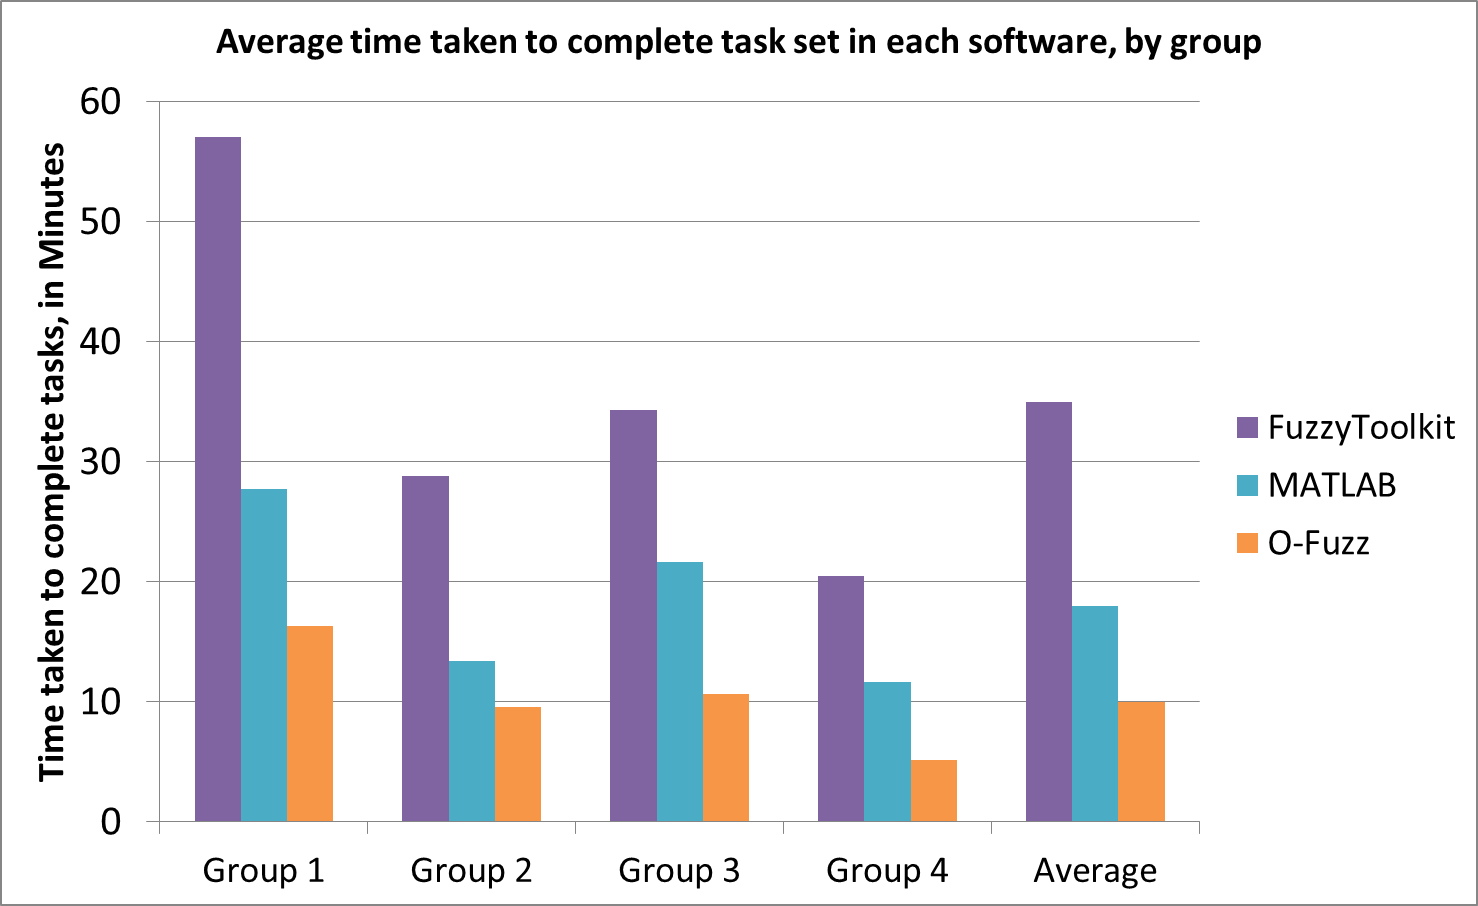
\includegraphics[width=0.8\textwidth]{images/timeTaken}
	\end{center}
	\vspace{-5mm}
	\captionsetup{justification=centering,margin=2cm}
	\caption{Bar chart of average time taken to complete the task set in the different software systems, by group}
	\label{fig:times}
	\vspace{-10mm}
\end{figure}
\newpage 
\noindent 						
Whilst the time taken to complete the tasks was a strong indicator of the success of the software system, it was also important to ask the participants which system they \emph{enjoyed} using the most. The results for this were conclusive, with 95.7\% of participants (across all categories) claiming FuzzyToolkitUoN was the piece of software they enjoyed using the least. The main reasons for this were the command line interface being difficult to use, visualisations of the system difficult to access, the necessity to constantly refer to the large documentation manual, and that it was conceptually confusing for many computer novices. 

\begin{figure}[ht!]
	\begin{center}
		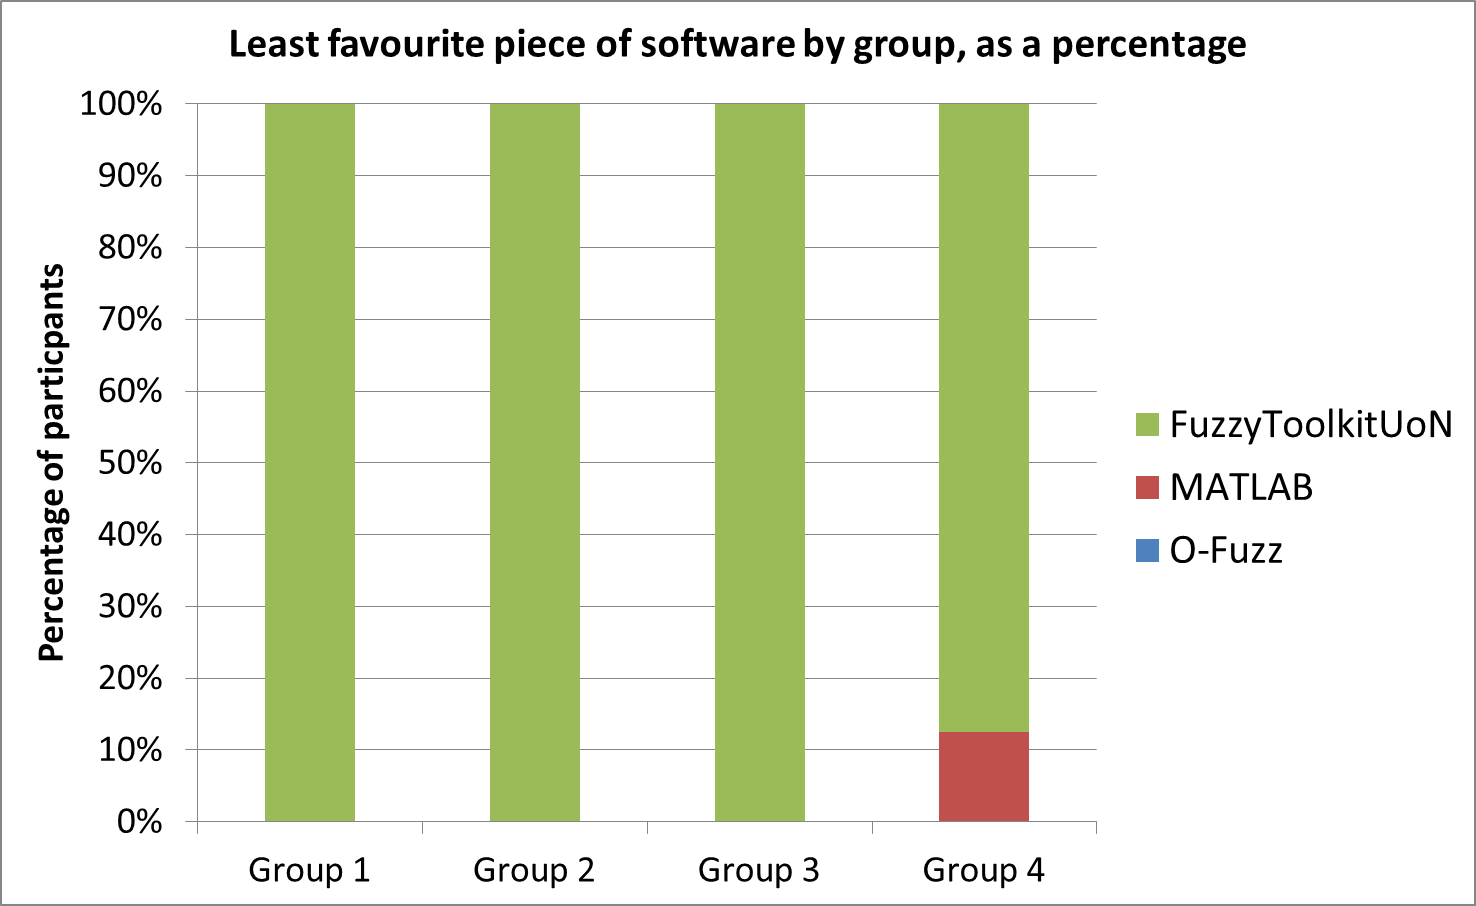
\includegraphics[width=0.8\textwidth]{images/leastFav}
	\end{center}
	\vspace{-5mm}
	\captionsetup{justification=centering,margin=2cm}	
	\caption{The percentage of users claiming each piece of software to be their least favourite}
	\label{fig:leastFavour}
	\vspace{-2mm}
\end{figure}
\noindent 
The piece of software that was most favoured by the test participants, was the system proposed in this report, o-Fuzz. Of the total participants, 65\% claimed o-Fuzz to be their favourite software, with 30\% saying it was MATLAB, and 4\% saying FuzzyToolkitUoN (a single person). A decomposition of favourite software, across the separate groups, can be seen in figure \ref{fig:mostLiked}
			
\begin{figure}[ht!]
	\begin{center}
		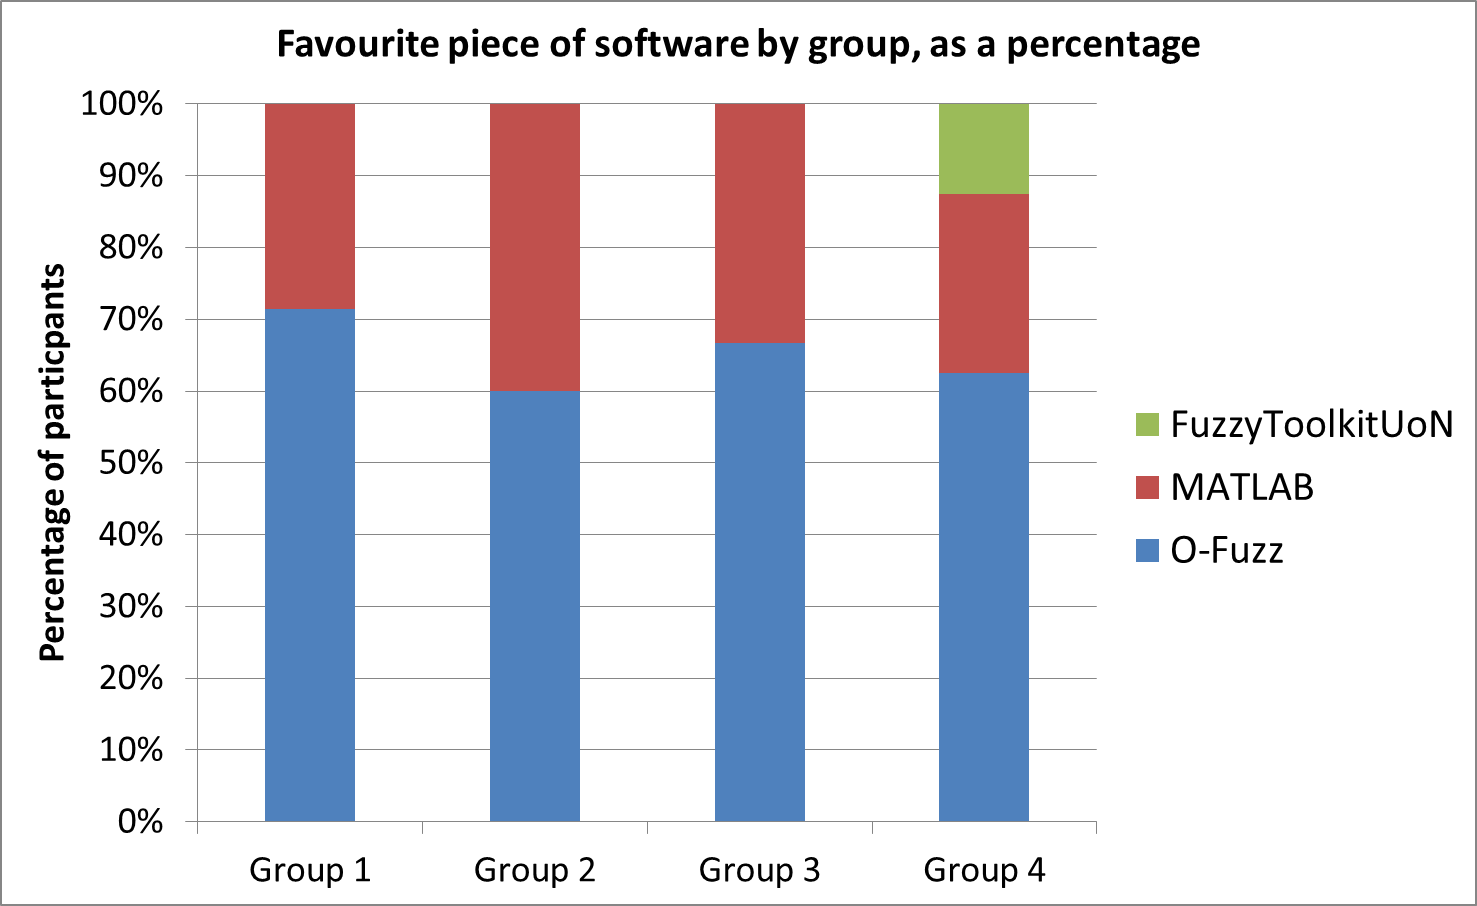
\includegraphics[width=0.8\textwidth]{images/mostFav.png}
	\end{center}
	\vspace{-5mm}
	\captionsetup{justification=centering,margin=2cm}	
	\caption{The percentage of users claiming each piece of software to be their most favourite}
	\label{fig:mostLiked}
	\vspace{-2mm}
\end{figure}
\noindent 
When questioned as to the preference of this new system, most users agreed that the interface was both extremely simple to navigate, and visually appealing. It was also mentioned that there was a natural flow to the software. By this, they meant that each task in the software lead onto the next very intuitively. For instance, the adding of a variable would be one distinct task, but the adding of membership functions would be a separate task nested inside this task. This meant that the conceptually distinct parts of the system were separate, but the system had a ``waterfall'' style flow to it. Many of the novice users also commended the system on it's help system, specifically mentioning how this was much more intuitive than checking the huge documentation manual provided with FuzzyToolkitUoN.\ \\
\ \\
It is worth noting that the single result for FuzzyToolkitUoN as favourite software came from a user that was extremely proficient in R, and specifically FuzzyToolkitUoN, and knew many commands from memory. This was also the same person that rated MATLAB as their least favourite piece of software, claiming that it was far too cluttered and aesthetically unappealing.
	

\subsection{Successes and Limitations of the Project}
Whilst getting user feedback is extremely important in evaluating a system, it is equally important for the creator of a software system to analyse the work they have completed. They are the only person that truly knows whether or not the software they have produced is what they were originally attempting to create. In this section, the successes and failures of the project have been listed, as seen by the project creator.\ \\
\ \\
The biggest strength of the project is its adherence to its two main goals: ease of use, and ease of accessibility. The purpose of this project was to both be a practical implementation of a fuzzy logic software system and, more specifically, open up the field of fuzzy logic to novices of the area, and novices in using computers in general. In this regard, the project was a huge success. The feedback received from the user feedback evaluation strongly suggested that this newly produced system performed much better than existing systems, and that it was much easier for novice users to pick up and understand. Further adding to the the system's accessibility, it was designed entirely in Bootstrap, meaning it was fully responsive, and would display adequately, regardless of the screen size of the user (in contrast to many systems nowadays that assume users have a certain level of space, which they may not always have). It was also more visually appealing as a result of the adoption of Bootstrap.\ \\
\ \\
The system has also been designed in such a way, that it is hopefully easily expandable in the future, and open to modification. One goal would be, eventually, the ability to swap the back end that the system used. This would be a relatively simple goal, as the system has been created so that the majority of tasks are a front end affair, and adoption of ``hot-swappable'' back ends would only require the implementation of some API layer between the front end and back end. The code base itself should also be relatively easy to add to and modify, due to the JavaDoc style comments that accompany every function in the system, that detail what the functions does, what parameters it expects (and their types), and what value the function returns - if any.
\newpage 
\noindent 
The final main strength of this new software system is the way that it deals with mistakes the user makes. Some systems (such as FuzzyToolkitUoN) provide extremely obtuse error messages that make the rectification of errors very difficult to the novice user. The system specified in this report implements errors message that are concise, but also explain the problem, and are worded in such a way that a solution can easily be inferred by the user (regardless of their skill level).\ \\
\ \\
As with any software project, there are obviously areas where extra work could have been completed to improve the system. The largest limitation of this new software system, is in fact, it's back end. Due to the relatively limited scope of the functionality of FuzzyToolkitUoN, the functionality for this new software system is also severely limited. Luckily, however, FuzzyToolkitUoN is still in development and extra functionality may become available, thus allowing extensions for this project. However, if extra time was allocated to this project, an API layer would have been implemented between the front end and any possible back end. This would then allow the back end to tell the front end what functionality it should expect, and the user would be able to swap the back end to whichever most closely met their needs.\ \\
\ \\
Another limitation with the software, that is present in any large software system, is the potential for some unidentified bug being present. Whilst the utmost has been done to ensure there are as few bugs as there can be, it is not always possible to claim there are none. This could have been helped, if Unit Testing and Test Driven Development were adopted towards the start of the project. This is the process of writing a test, and writing the code necessary to pass the test. This ensures that all code written is free of bugs, is as concise as possible, and integration and regression tests are extremely easy to perform\cite{olan2003unit} (as all the tests from previous work still remain).\ \\
\ \\
The final limitation of the project, which was noted when testing the responsiveness of the software, is that the system does not load or display correctly on mobile devices. This is mostly due to Bootstrap, and how modal windows in Bootstrap (that are heavily used throughout the software) do not render correctly properly on mobile devices. Luckily, this isn't truly an issue, as the project was never intended to work on mobile devices, as this is an impractical medium in which to construct a fuzzy system, and thus no actions would be taken to amend this.

\newpage 
\section{Further Work}
The system that was produced adhered to all of the functional requirements that the client laid out at the beginning of the project, but that does not mean that all potential functionality has been implemented, or even that the system is truly complete. In this section three key areas of functionality have been identified and expanded upon, and provide a starting point for the maintainers of the software to focus on.\ \\
\ \\
The first of these areas is the routing system, specifically how the route between two points is calculated. Currently, the user is the main factor influencing how scenic a route is. It is expected they will select several key picturesque locations, and the drive between them will also be pleasant. However, this will not always be the case, and a good route could be spoiled with the transitions between two points, especially if the distance between the points is large. The reason for this is that the routing system provides the shortest path between any two selected points, rather than the most visually appealing. In future iterations of the project, it would be beneficial if some data mining was performed alongside the routing system, so that multiple routes could be generated, their pleasantness evaluated, allowing the system to pick the best looking journey. This would improve the quality of all the routes in the system, as well as further helping to achieve the main goal of the application: to improve the user's driving experience.\ \\
\begin{figure}[!ht]
	\vspace{-3mm}
	\begin{center}
		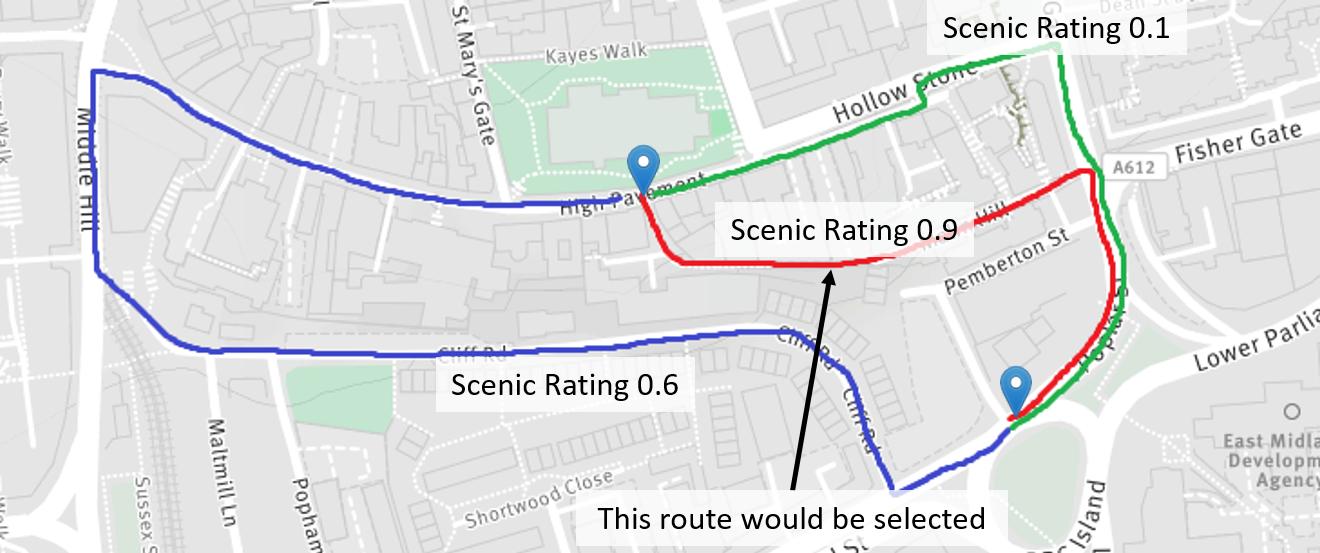
\includegraphics[width=0.9\textwidth]{images/further/alt.png}
	\end{center}
	\vspace{-6mm}
	\caption{Route recommendation based on some scenic rating}	
\end{figure}
\ \\
The next area of future expansion would be the social interaction system. As it stands, the system provides support for users to have six interactions with routes: commenting, rating, sharing, downloading, cloning, and recommending similar routes. This is fine for users that don't use the site frequently, or don't visit a lot of routes, but for dedicated and recurrent users, it quickly becomes apparent there are some issues with managing their social interactions. There is no one central place where a user can view all the interactions that other users have had with them. This means that if a user wants to keep a track of this, they have to religiously check their emails, or visit each of their routes individually, which becomes much more difficult the more routes and interactions the user has. The solution to this problem is to implement some form of notification centre, where a user can see all the notifications they have received, similar in functionality to the notification system employed by Facebook. 

\newpage 
\noindent 
This would allow for users to review all of their notifications in a centralised place, so that they do not miss any, and do not need to check multiple locations for their notifications (which would not scale well as the number of sources of notifications, their routes, increases). This could then be further expanded with the ability to follow routes and other users of the system, so that notifications could be received for these as well.

\begin{figure}[!ht]
	\begin{center}
		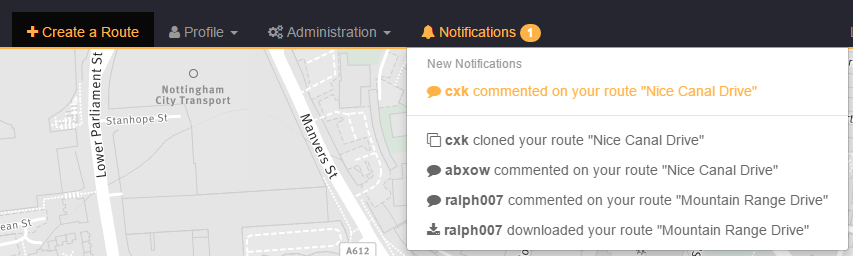
\includegraphics[width=0.95\textwidth]{images/further/notification.png}
	\end{center}
	\vspace{-6mm}
	\caption{Mock up of the notification system, displaying all social interactions received}	
\end{figure}

\noindent 
The final area of further work is also an improvement on social interactions within the site, specifically the implementation of a site wide messaging system. This would allow for users to interact with one another on a much more personal level than simply commenting on each others routes. This deeper social interact could become one of the main driving features for users to returning to the site. It provides the ability for users to talk to users that provide quality content, friendships to form, and for groups with similar interests to develop. It would also mean that communication between members would be contained within the Niceway.to ecosystem, rather than users communicating on other social platforms, and potentially missing out on what's happening with their friends on Niceway.to. This freedom to communicate with other users would open up a lot of potential for Niceway.to and would increase the chance of users returning to the site on a regular basis (to check for any new messages).

\begin{figure}[!ht]
	\begin{center}
		
\includegraphics[width=0.9\textwidth]{images/further/chat.png}
	\end{center}
	\vspace{-6mm}
	\caption{Mock up of the chat system}	
\end{figure}
\newpage 
\section{Summary \& Personal Evaluation}
{\color{red}
	\begin{itemize}
		\item Personally, I feel as thought the project was a /success$\mid$failure/
		\item I felt as though I /failed to rise$\mid$rose/ to the challenge
		\item One of the areas I feel as though was weaker within the project
		\item If I could work on this project again
	\end{itemize}
}




%
%
% Bibliography
%
%

\newpage
\pagestyle{biblio}
\bibliographystyle{plain}

\bibliography{bib}


%
%
%  Appendix 
% 
%
\newpage
\pagestyle{appendix}
\appendix
\section{Initial System Designs}
\label{sec:isd}
\subsection{Route Discovery/Landing Page}
\begin{figure}[!ht]
    \begin{center}
        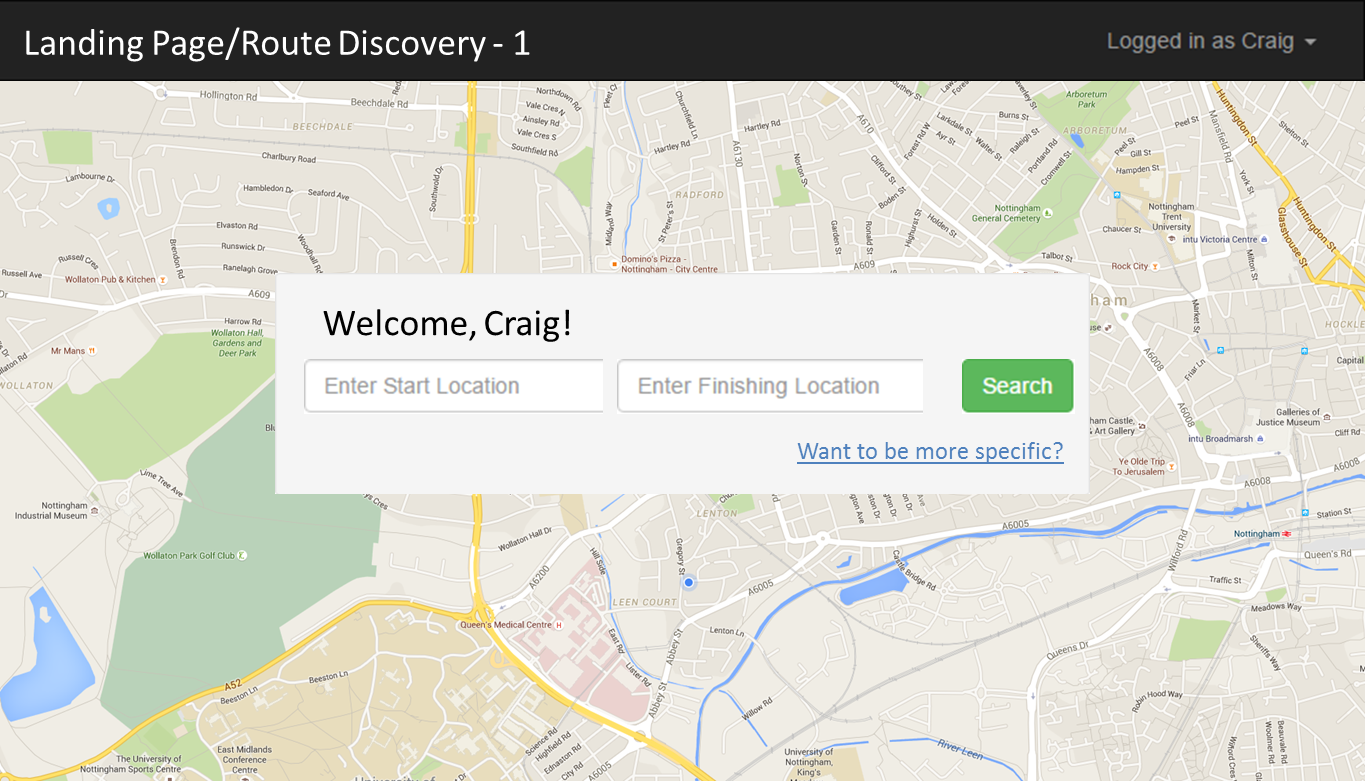
\includegraphics[width=0.725\textwidth]{images/appendix/landing1.png}
    \end{center}
    \vspace{-6mm}
\end{figure}

\begin{figure}[!ht]
    \begin{center}
        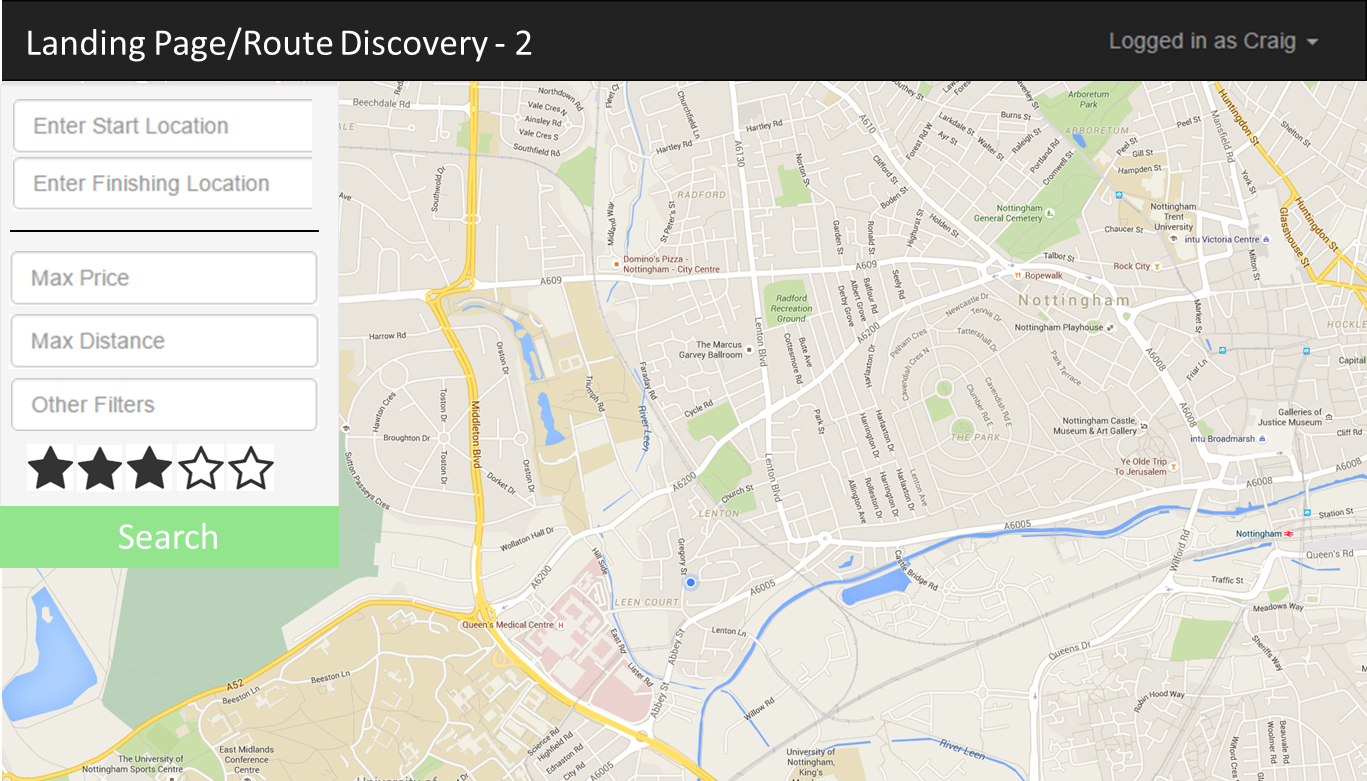
\includegraphics[width=0.725\textwidth]{images/appendix/landing2.png}
    \end{center}
    \vspace{-6mm}
\end{figure}

\begin{figure}[!ht]
    \begin{center}
        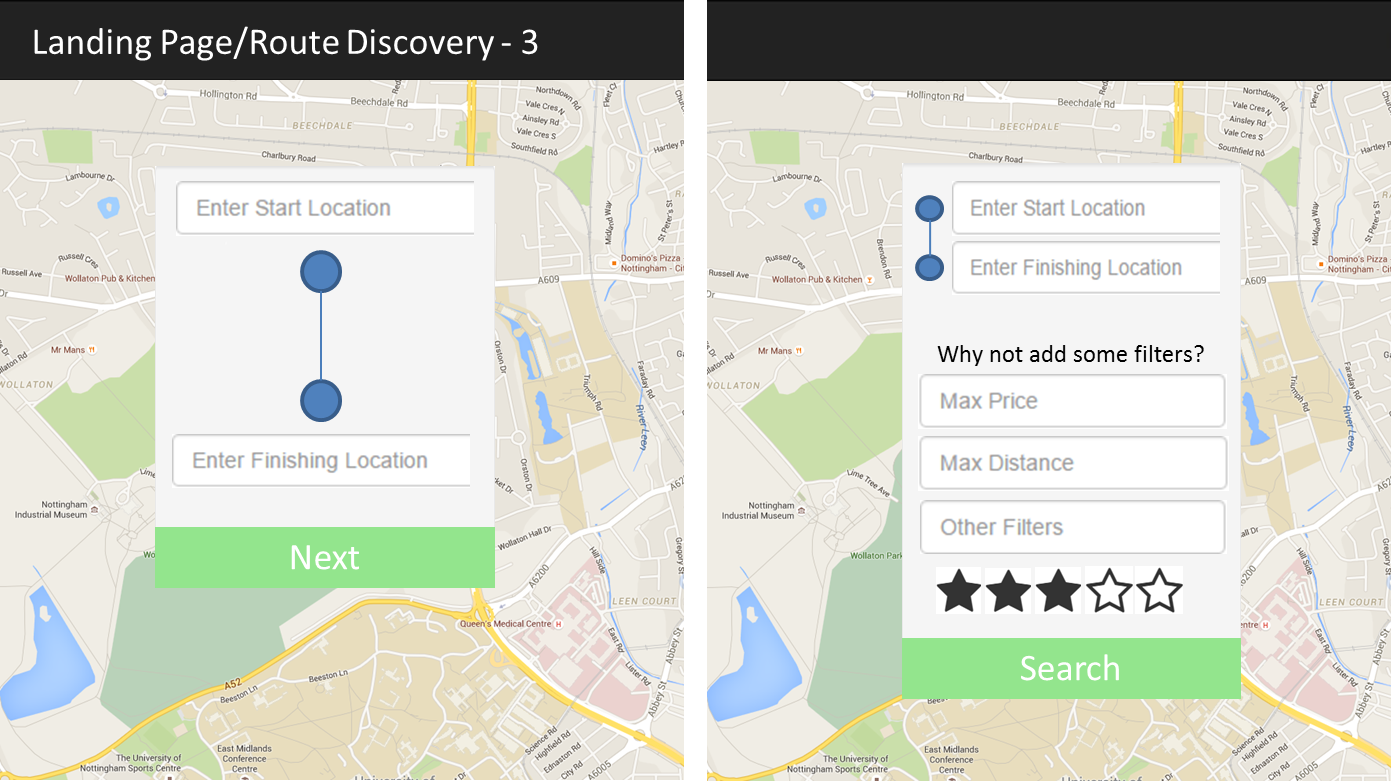
\includegraphics[width=0.725\textwidth]{images/appendix/landing3.png}
    \end{center}
    \vspace{-6mm}
\end{figure}

\newpage 
\subsection{Route Listing Page}
\begin{figure}[!ht]
    \begin{center}
        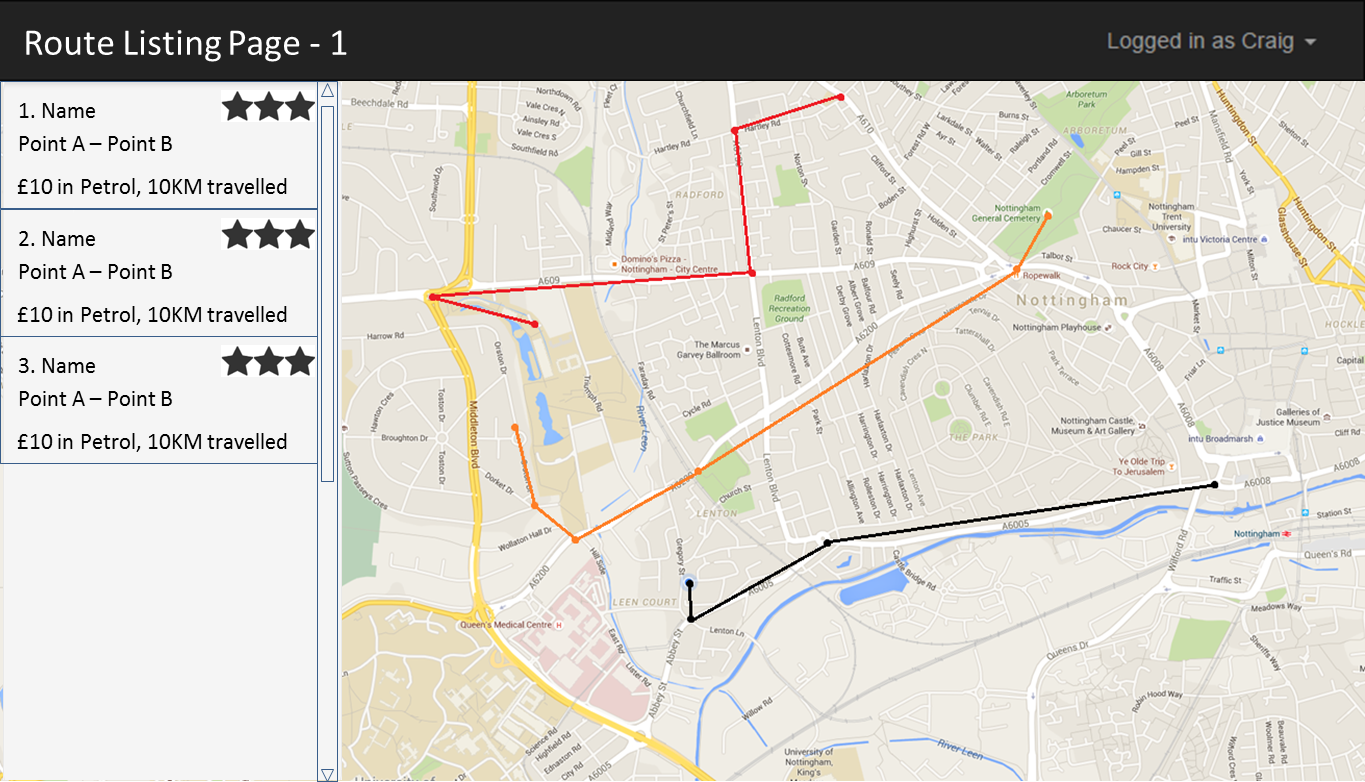
\includegraphics[width=0.75\textwidth]{images/appendix/rlp1.png}
    \end{center}
    \vspace{-6mm}
\end{figure}

\begin{figure}[!ht]
    \begin{center}
        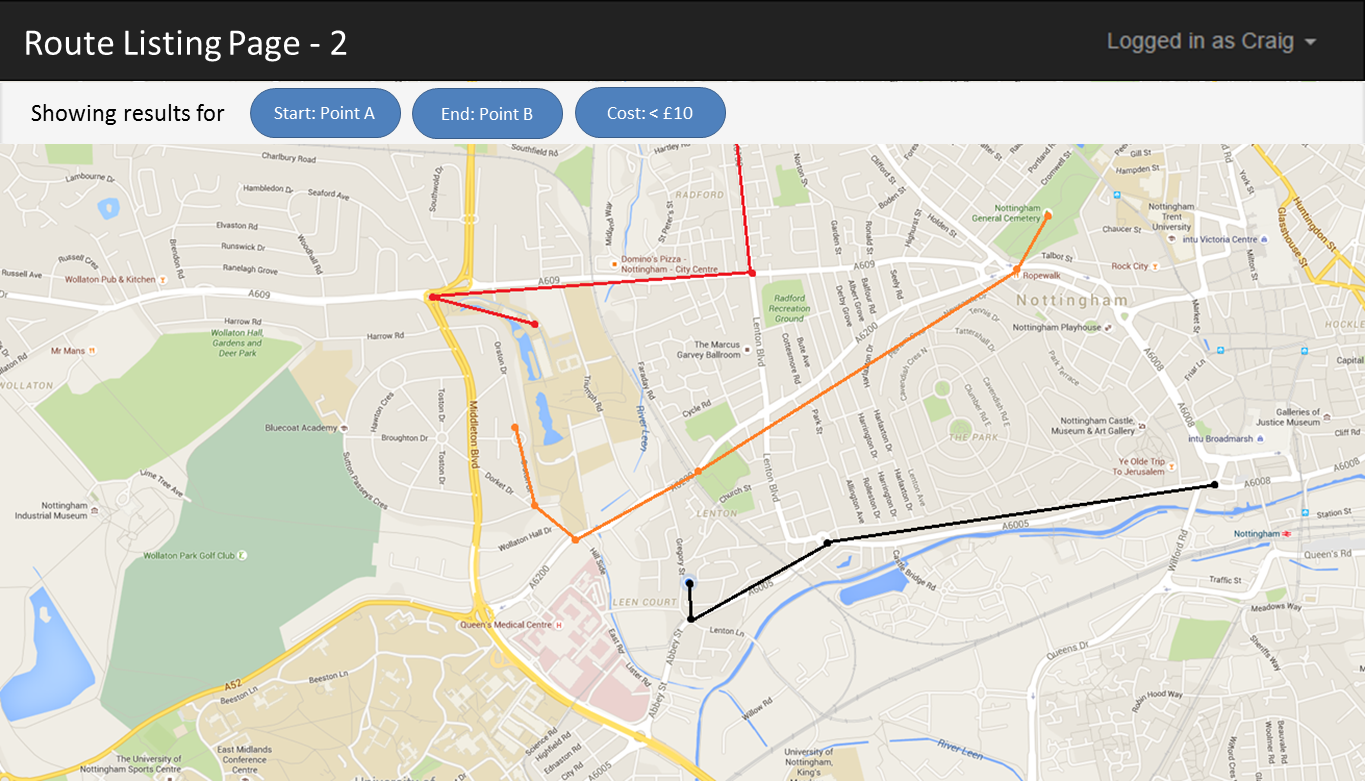
\includegraphics[width=0.75\textwidth]{images/appendix/rlp2.png}
    \end{center}
    \vspace{-6mm}
\end{figure}

\begin{figure}[!ht]
    \begin{center}
        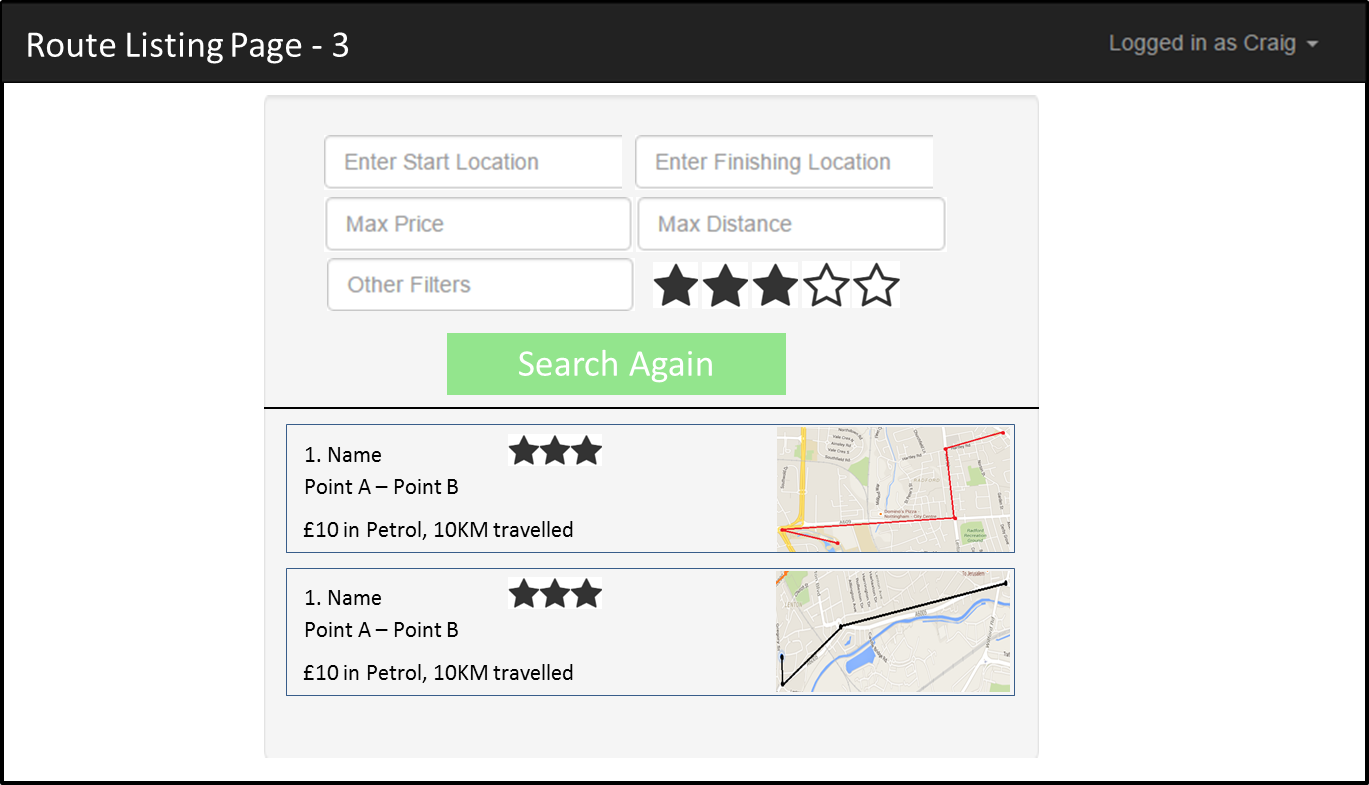
\includegraphics[width=0.75\textwidth]{images/appendix/rlp3.png}
    \end{center}
    \vspace{-6mm}
\end{figure}

\newpage 
\subsection{Route Detail Page}
\begin{figure}[!ht]
    \begin{center}
        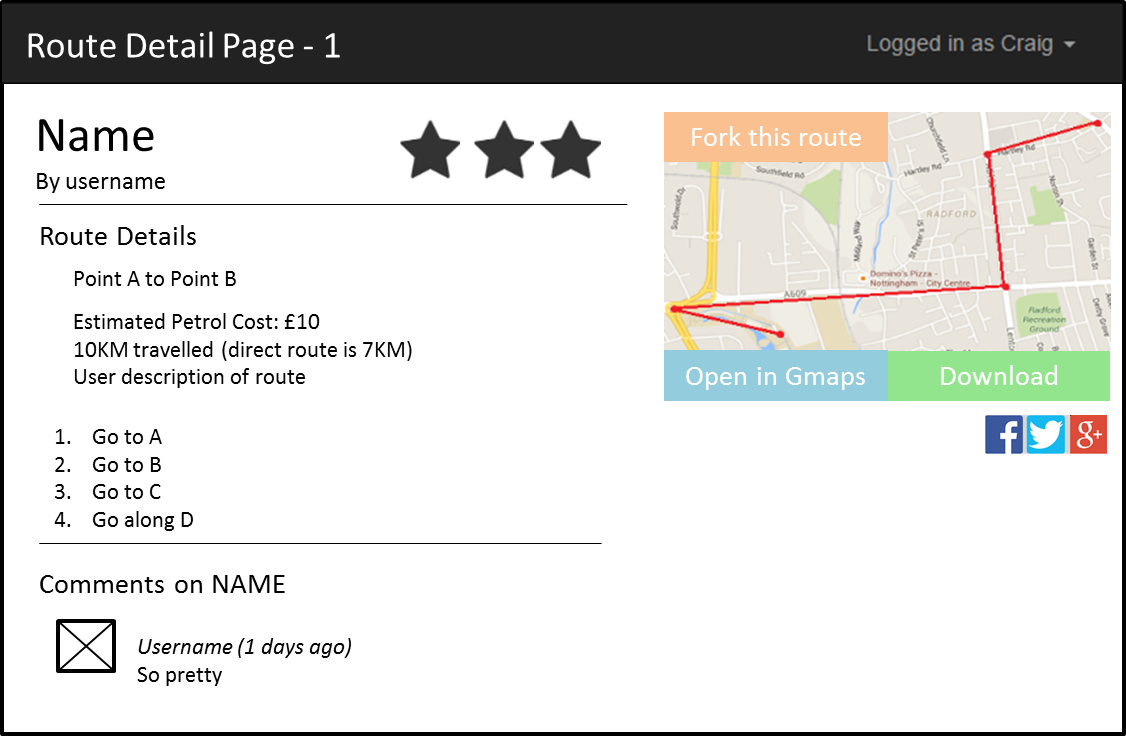
\includegraphics[width=0.75\textwidth]{images/appendix/rdp1.png}
    \end{center}
    \vspace{-6mm}
\end{figure}

\begin{figure}[!ht]
    \begin{center}
        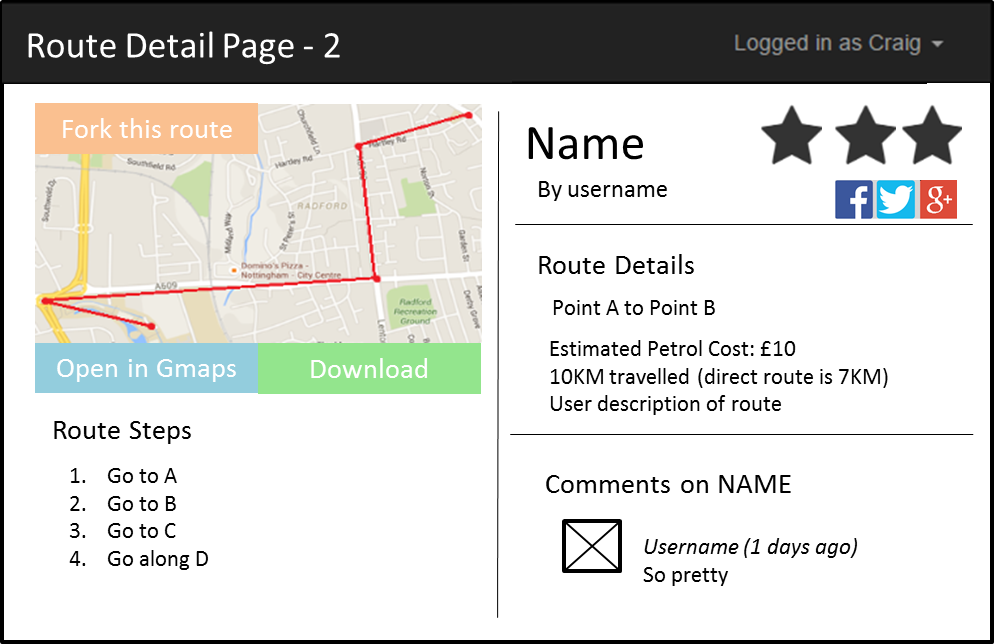
\includegraphics[width=0.75\textwidth]{images/appendix/rdp2.png}
    \end{center}
    \vspace{-6mm}
\end{figure}

\begin{figure}[!ht]
    \begin{center}
        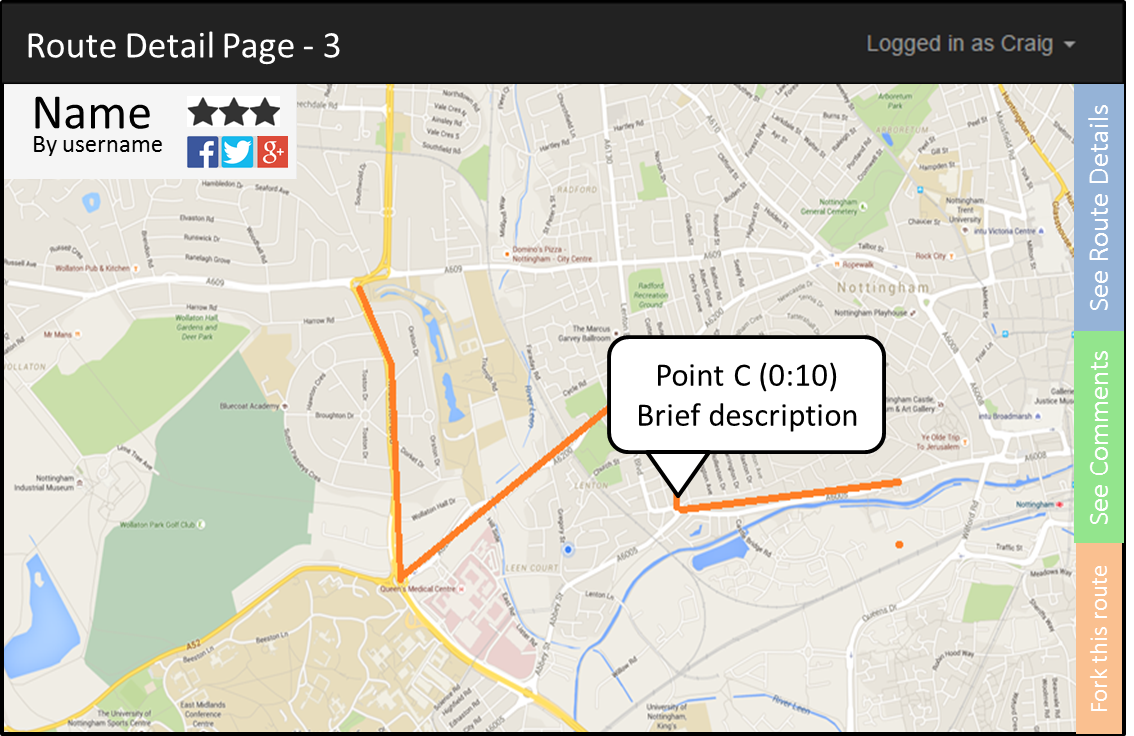
\includegraphics[width=0.75\textwidth]{images/appendix/rdp3.png}
    \end{center}
    \vspace{-6mm}
\end{figure}

\subsection{Route Creation Page}
\begin{figure}[!ht]
    \begin{center}
        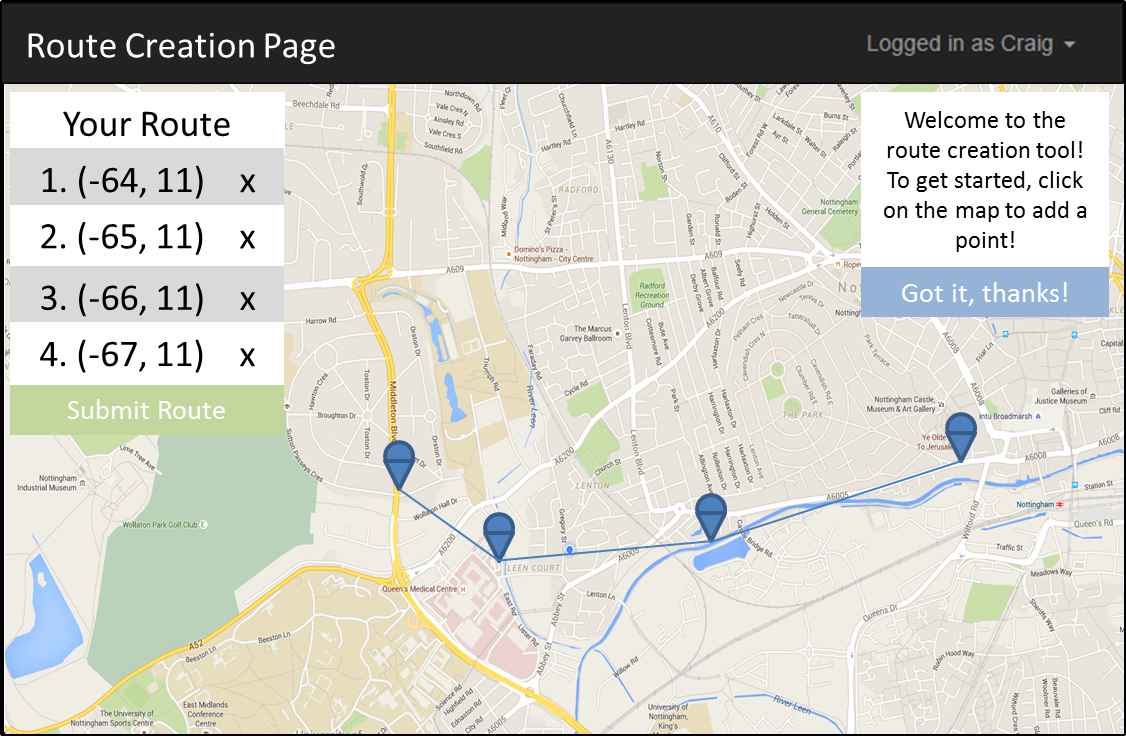
\includegraphics[width=0.8\textwidth]{images/appendix/rcp1.png}
    \end{center}
    \vspace{-6mm}
\end{figure}

\subsection{Profile Page}
\begin{figure}[!ht]
    \begin{center}
        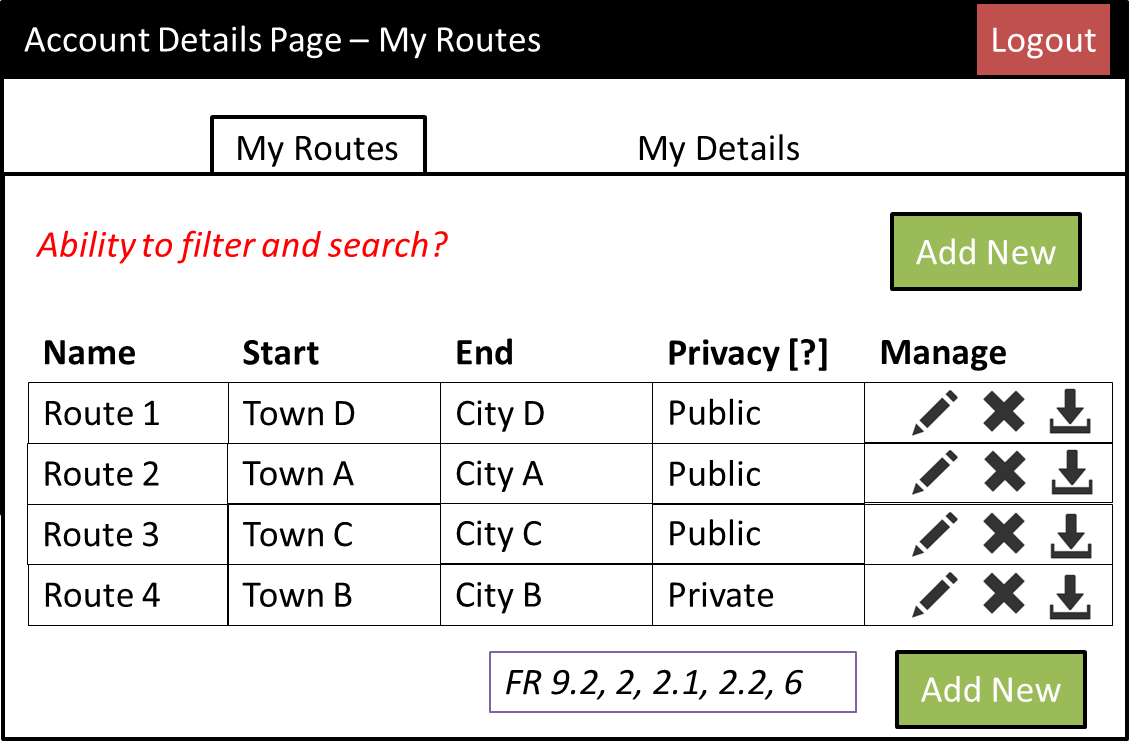
\includegraphics[width=0.8\textwidth]{images/appendix/prof1.png}
    \end{center}
    \vspace{-6mm}
\end{figure}


\newpage 
\section{Interface Design Heuristics}
\label{sec:idh}

\subsection{Jakob Nielsen's Usability Heuristics}
\begin{enumerate}
    \item Visibility of system status
    \item Match between system and the real world
    \item User control and freedom
    \item Consistency and standards
    \item Error prevention
    \item Recognition rather than recall
    \item Flexibility and efficiency of use
    \item Aesthetic and minimalist design
    \item Help users recognize, diagnose, and recover from errors
    \item Help and documentation
\end{enumerate}

\subsection{Ben Schneiderman's Golden Rules}
\begin{enumerate}
    \item Strive for consistency.
    \item Enable frequent users to use shortcuts.
    \item Offer informative feedback.
    \item Design dialog to yield closure.
    \item Offer simple error handling.
    \item Permit easy reversal of actions.
    \item Support internal locus of control.
    \item Reduce short-term memory load.
\end{enumerate}


\newpage 
\newgeometry{left=15pt,right=20pt,top=30pt,bottom=20pt}
\pagestyle{none}
\begin{landscape}
\section{Project Gantt Chart}
\label{sec:gantt}
	\begin{center}
		\begin{ganttchart}[
			y unit chart = 0.6cm,
			y unit title = 0.6cm,
			x unit = 0.6cm,
			vgrid,
			hgrid,
			Mile1/.style={milestone/.append style={fill=green}},
			Mile2/.style={milestone/.append style={fill=red}}
			]{1}{32}
			\gantttitle{Project Time Plan}{32}\\ 
			\gantttitlelist{"Oct"}{4}
			\gantttitlelist{"Nov"}{5}		
			\gantttitlelist{"Dec"}{4}	
			\gantttitlelist{"Jan"}{4}
			\gantttitlelist{"Feb"}{5}
			\gantttitlelist{"Mar"}{4}			
			\gantttitlelist{"Apr"}{4}	
			\gantttitlelist{"May"}{2}\\
			\gantttitlelist{5, 12, 19, 26,
				2, 9, 16, 23, 30,
				7, 14, 21, 28,
				4, 11, 18, 25,
				1, 8, 15, 22, 29,
				7, 14, 21, 28,
				4, 11, 18, 25,
				2, 9
			}{1}\\
			\ganttset{progress label text={},
				bar incomplete/.append style={fill=green!40},
				group/.append style={draw=black, fill=green},}
			\ganttgroup{Documentation}{1}{28} \\
			\ganttbar[progress=0]{1. Design Specification}{1}{1}\\ 					%0
			\ganttbar[progress=0]{2. Initial Project Plan}{2}{2}\\						%1
			\ganttmilestone[Mile1]{Initial Project Plan Deadline (17th)}{2}\\	%2	
			\ganttbar[progress=0]{3. Revised Project Plan}{4}{4}\\						%4
			\ganttmilestone[Mile1]{Revised Project Plan Deadline (2nd)}{4}\\	%5				
			\ganttbar[progress=0]{4. Write Dissertation}{25}{28}\\						%17
			\ganttmilestone[Mile1]{Hand-in Dissertation (18th)}{28}\\			%18

			\ganttset{progress label text={},
				bar incomplete/.append style={fill=blue!40},
				group/.append style={draw=black, fill=blue},}
			\ganttgroup{Development}{5}{23} \\											
			\ganttbar[progress=0]{5. Sign Up Page (A1, O4)}{5}{5}\\								%6
			\ganttbar[progress=0]{6. Log In Page (A1, O2)}{5}{5}\\								%7
			\ganttbar[progress=0]{7. My Details Page (O4)}{5}{5}\\							%8
			\ganttbar[progress=0]{8. Route Creation Page (O2)}{6}{7}\\						%9
			\ganttbar[progress=0]{9. My Routes Page (O4)}{9}{9}\\							%13
			\ganttbar[progress=0]{10. Route Detail Page (O3, O6)}{10}{11}\\						%14
			\ganttbar[progress=0]{11. Route Discovery Page (O1)}{17}{18}\\					%13
			\ganttbar[progress=0]{12. Route Listing Page (O1)}{19}{20}\\						%15
			\ganttbar[progress=0]{13. Admin Page and Functionality (O5)}{21}{23}\\			%16
		
			\ganttset{progress label text={},
						bar incomplete/.append style={fill=red!40},
						group/.append style={draw=black, fill=red},}
			\ganttgroup{Misc. Tasks}{3}{31} \\						
			\ganttbar[progress=0]{14. Set up database structure}{3}{3}\\				%3
			\ganttbar[progress=0]{15. Set up web hosting and repository}{3}{3}\\		
			\ganttbar[progress=0]{16. Add Test Routes}{8}{8}\\							%11			
			\ganttbar[progress=0]{17. Prepare for demonstration}{30}{31}\\				%19	
			\ganttmilestone[Mile2]{Demonstration (3rd-5th)}{31}\\				%20
					
		\ganttset{progress label text={},
			bar incomplete/.append style={fill=purple!40},
			group/.append style={draw=black, fill=purple},}
		\ganttgroup{Other Commitments}{6}{16} \\											
		\ganttbar[progress=0]{18. Other Coursework Deadlines}{6}{8}\\	
		\ganttbar[progress=0]{19. Exam Revision/Final Courseworks}{11}{16}\\		%14    
	\end{ganttchart}
	\end{center}
\end{landscape}

\newpage
\restoregeometry
\newgeometry{left=3cm, right=3cm, top = 75pt, bottom=75pt}
\pagestyle{appendix}





%
%
% Qed
%
%

\end{document}	